\documentclass{report}

%--------------------------------------------------- PAGE STYLE 
\usepackage[utf8]{inputenc} 		% Encoding
\usepackage[T1]{fontenc} 			% To write in French
\usepackage[english]{babel} 		% To write in English
\usepackage{fancyhdr} 				% Fancy style
\usepackage[left=1.7cm,right=1.7cm,top=1.7cm,bottom=1.7cm]{geometry}
\usepackage[titletoc]{appendix}	   	% Better appendix management
\usepackage[absolute]{textpos}
\usepackage{booktabs}

\usepackage{expdlist}
\newenvironment{itemize*}%			% Creates a custom itemize environment, called by itemize* 
  {\begin{itemize}%
    \setlength{\itemsep}{0pt}%		% The interline is reduced so that we don't waste space
    \setlength{\parskip}{0pt}}%
  {\end{itemize}}
  
\renewcommand{\rmdefault}{phv}		% Use Helvetica as default font for the whole document

\setlength{\parindent}{0pt}	      	% Remove auto-ident

%--------------------------------------------------- COOL CHAPTER NUMBERING
\usepackage{titlesec, blindtext, color}

\titlespacing*{\chapter}{0pt}{0pt}{20pt}	% Remove space used by the "chapter" header

\definecolor{black}{gray}{0}
\newcommand{\hsp}{\hspace{20pt}}
\titleformat{\chapter}[hang]{\LARGE\bfseries}{\thechapter\hsp\textcolor{black}{|}\hsp}{0pt}{\LARGE\bfseries}

%--------------------------------------------------- BIBLIOGRAPHY 
\usepackage{natbib}

%--------------------------------------------------- MATHS STUFF 
\usepackage{float}					% For float
\usepackage{amsmath,amscd,amssymb,epsfig}  %sci equations
\usepackage{matlab-prettifier}      % MATLAB codes
\usepackage[numbered,framed]{mcode} % For MATLAB code
\usepackage{verbatim}               % to quote code
\usepackage{listings}               % Include the listings-package
\usepackage{lipsum}					% Cite code
\usepackage{tocloft}				% Different codes inputs manager (python, SciLab, ...)

%--------------------------------------------------- INCLUSIONS 
\usepackage{array}					% Required for tabulars 
\usepackage{graphicx} 				% Required for the inclusion of images
\usepackage{wrapfig}			    % To make wrapped figures 
\usepackage[format=plain,
			font={small},
			labelfont={bf,it},
			textfont=it]{caption}   % To include captions (small, figure in bold, all text in italic)
\usepackage{enumitem}               % To make lists
\usepackage{url}                    % to quote URLs
\usepackage{pdfpages}			    % To include PDFs (annexes)
\usepackage{textcomp}		        % For copyright symbol
\usepackage{hyperref}				% To make references 


%--------------------------------------------------- CUSTOM COMMANDS
\newcommand{\ts}{\textsuperscript} 	% Simplifies superscript
\newcommand{\tsb}{\textsubscript}  	% Simplifies subscript

% define list of equations
\newcommand{\listequationsname}{List of Equations}
\newlistof{myequations}{equ}{\listequationsname}
\newcommand{\myequations}[1]{%
\addcontentsline{equ}{myequations}{\protect\numberline{\theequation}#1}\par}
\setlength{\cftmyequationsnumwidth}{2.5em} % Width of equation number in List of Equations
\setlength{\cftmyequationsindent}{1.5em}   % Indent of list of equation 

 
\begin{document}

%---------------------------------------------------------------------
%	TITLE PAGE
%---------------------------------------------------------------------

\begin{titlepage}

\newcommand{\HRule}{\rule{\linewidth}{0.5mm}} % horizontal lines

\center % Center everything on the page


\includegraphics[scale=0.4]{logo.png} \\[3cm] % Logo

	%	HEADING 

\textsc{\large International Master Degree in Electro-Acoustics, 2\ts{nd} Year internship report}\\[0.4cm] % Major heading 
\textsc{\normalsize Academic year 2017 - 2018}\\[0.7cm] % Minor heading 

	%	TITLE 

\HRule \\[0.4cm]
 { \huge \bfseries Near-Field Scanner: measurement optimization}\\[0.3cm] 
\HRule \\[1.5cm]

	% DATE
    
{\large \today}\\[2cm] 

	%	AUTHORS - SUPERVISORS

\begin{minipage}{0.4\textwidth}
\begin{flushleft} \large
\emph{Author:}\\ % Author(s)
Chlo\'{e} \textsc{Corno}

\end{flushleft}
\end{minipage}
~
\begin{minipage}{0.4\textwidth}
\begin{flushright} \large
\emph{Referees:} \\ % Supervisor(s) 
\textit{Academic:} Manuel Melon \\
\textit{Company:} Christian Bellmann \\

%\emph{Reviewer:} \\ % Reviewer Name

\end{flushright}
\end{minipage}\\[2cm]
 
\vfill % Fill the rest of the page with white

\end{titlepage}

%---------------------------------------------------------------------
%	THANKS
%---------------------------------------------------------------------

\chapter*{}
\thispagestyle{empty}
\begin{center}
{\Large\textbf{Acknowledgements}} \\~\\~\\~\\
\end{center}

I would first like to thanks my supervisor Chrisitan Bellmann for all the help and support he provided me during these 5 months. \\

I want to particularly thanks the Université du Mans and all the professors and supervisors for giving me the opportunity to follow the Internal Master Degree in ElectroAcoustics and allowing me to work in a domain that passionate me. \\

I would also like to acknowledge Valentin Binet, for all the support and love he provided since he knows me; and as the second reader of this report. I am gratefully indebted to him for his very valuable comments on this report.\\

Finally, I want to express my profound gratitude to my family who supported me during my studies. I would've never made it without you. Thank you.

\newpage
%---------------------------------------------------------------------
%	TABLE OF CONTENTS - LIST OF FIGURES
%---------------------------------------------------------------------
\pagenumbering{alph} % aplha page numbering for ToC and LoF

\clearpage
	% Change the name of table of contents and other lists
\renewcommand\contentsname{Table of contents}
\tableofcontents
\addtocontents{toc}{~\hfill\textbf{Page}\par} % Adds "page" on top of page number

\clearpage
\listoffigures
\addcontentsline{toc}{chapter}{List of Figures}

\clearpage
\listofmyequations
\addcontentsline{toc}{chapter}{List of Equations}

%--------------------------------------------------------------
%	CODE SAMPLES
%--------------------------------------------------------------

	% IMAGE WITHOUT FLOAT 
    
%\begin{center}
%\includegraphics[width=\textwidth]{name_of_figure} 
%\captionsetup{hypcap=false} 
%\captionof{figure}{some caption for the figure} 
%\label{fig:name_of_label}
%\end{center}

	% EASY SUPRESCRIPT
    
 
%\newcommand{\ts}{\textsuperscript}  %write with usepackage

%1\ts{rst} 2\ts{nd} 3\ts{rd}  ....

	% ADD CONTENT TO ToC 
    
%\addcontentsline{toc}{[type]}{[Name]}
% type : chapter section subsection ...?
% Name : introduction, ...?

	% MINIMIZE SPACE BETWEEN LINES IN ITEMIZE
% \begin{itemize}
% 	\setlength\itemsep{1em}
% 	\item What is the influence of the position of the speaker?
% 	\item Can a mispositioned DUT be detected and adjusted?
% \end{itemize}

%--------------------------------------------------------------
%	INTRODUCTION
%--------------------------------------------------------------

\chapter*{Introduction}
\addcontentsline{toc}{chapter}{Introduction}
\pagenumbering{arabic} % Arabic page numbering for text corpus


"\textit{What defines a good measurement of a speaker?}" is a common rhetorical question for anyone working in the field of electroacoustics. While purely electrical measurements such as the impedance are quite immune to noise, they do not allow to fully characterize a driver, and acoustical measurements must be conducted. \\
A popular acoustical measurement for loudspeakers is the directivity: allowing to see how a driver radiates at a given angle, this measurement is usually done using one or an array of microphones, and by placing the Device Under Test on a turntable. By rotating the Device Under Test and measuring its SPL response for several angles, the directivity of the device is measured. \\

Although this method is widely used, it presents several drawbacks:
\begin{itemize}
\item Resolution: the higher the angular resolution, the better the measurement but the longer it takes. 
\item Accuracy: a good measurement must ideally be performed in an anechoic room, and in the far field of the Device to avoid any near field effects such as diffraction and interferences.
\item Price: the materials required such as an anechoic room or a performant microphone array can either very expansive or difficult to access. 
\end{itemize}




The following reports aims to present the work that have been conducted during a 5-months internship at the company Klippel GmbH. This internship is mandatory to graduate from the International Master Degree in Electro-Acoustics (IMDEA) at the Université du Mans, in France. \\

This document will cover different points, starting with a preface presenting the company, the context and aim of this work, and a literature review. Then the different measurements and results obtained during this work will be presented by using three topic: measurement of devices mounted in baffle, optimization of the measurement time of a device called the Near Field Scanner, and correction of measurements in bad room such as workshops. 


%--------------------------------------------------------------
%	PRESENTATION OF THE COMPANY ,  MISSION , LITTERATURE REVIEW
%--------------------------------------------------------------
\chapter{Preface}

	% COMPANY 
    
\section{Presentation of the company}

\begin{minipage}{0.35\textwidth}
\centering
	
\includegraphics[scale=0.2]{Preface/logo_klippel} 
    \captionsetup{hypcap=false} 
	\captionof{figure}{Logo of Klippel GmbH} 
	\label{fig:lolo_klippel}
\end{minipage}
\begin{minipage}{0.65\textwidth}
Founded in 1997 by Prof. Dr. Wolfgang Klippel from the T.U. Dresden, Klippel GmbH is a company specialized in the development of test equipment dedicated to electroacoustic transducers and audio systems, for both industry and laboratories. Thanks to many research and development, the company has created more accurate physical models for transducers, micro-speakers and headphones, valid for both small and large signals.  \\
Over the years, Klippel GmbH has acquired a huge notoriety for their innovative products but also thanks to many conferences and trainings. Their equipment is now used world-wide for measuring, testing, and designing loudspeakers.
\end{minipage}


	% CONTEXT, AIM OF THE WORK
    
\section{Context and aim of the work}

\begin{minipage}{0.6\textwidth}
The Near Field Scanner (NFS) is a Klippel product, shown in figure \ref{fig:nfs}, used to perform near field measurements of various audio products (laptop speakers, line arrays, ...). The particularity of this product is that the Device Under Test (DUT) is at a fixed position, and the microphone moves thanks to a robotic arm. This allows to ensure a constant interaction between the DUT and the acoustical boundaries, and avoid any diffraction from the edges of a turntable. \\

This works mainly aims to the redaction of several applications notes for Klippel's customers on the utilisation of the NFS with 3 main guidelines, which are the measurement of a speaker mounted on a baffle using the NFS; the optimization of measurement time by exploiting symmetries, and the application of room correction on this measurements.
\end{minipage}
\begin{minipage}{0.4\textwidth}
\begin{center}
	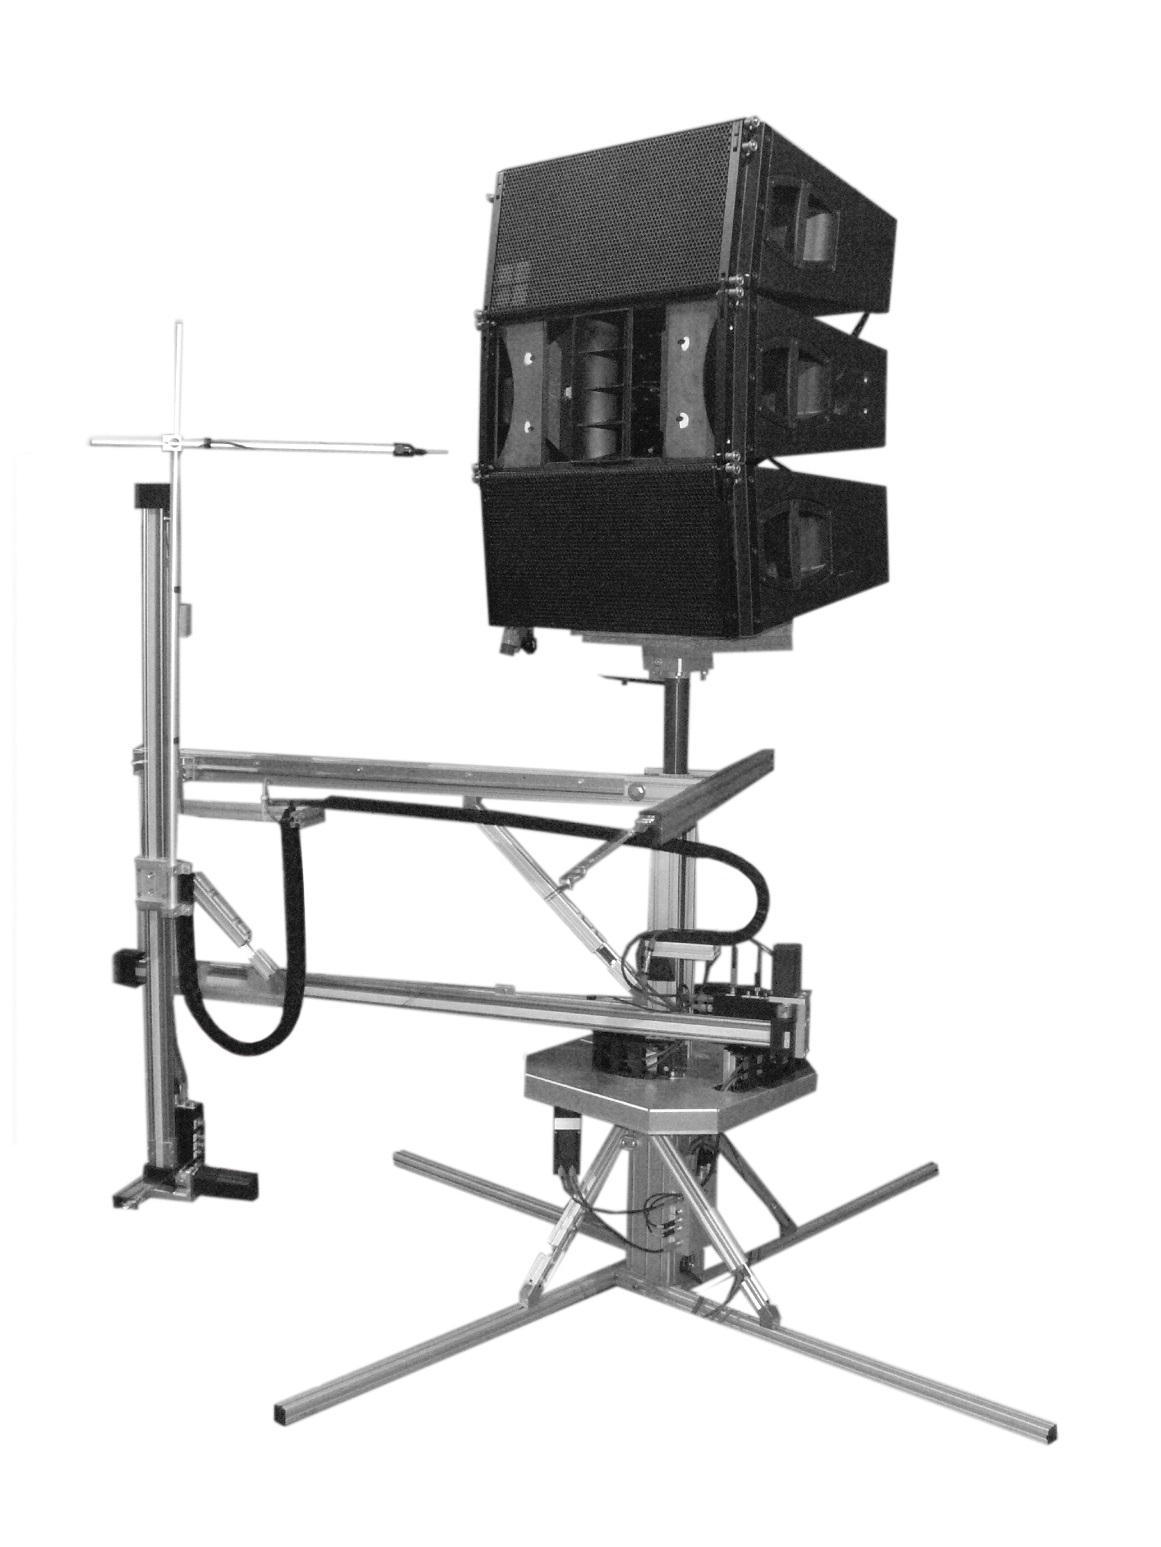
\includegraphics[scale=0.13]{Preface/NFS2} 
    \captionsetup{hypcap=false} 
	\captionof{figure}{Klippel Near Field Scanner} 
	\label{fig:nfs}
\end{center}
\end{minipage}\newline

The NFS baffle measurement aims to create several application notes on how to perform an near field scanning of a loudspeaker mounted on a baffle and evaluate the measurement error. To do so, the required tasks are the assembly and evaluation a baffle prototype, the optimization the measurement grid and of the measurement time by assuming symmetry conditions on the DUT.\\

The measurement time optimization part aims to reduce the scanning effort of the NFS by exploiting symmetry conditions on the complex coefficients of the spherical wave expansion (see equation \ref{eq:sphwvexp}). \\

The room correction part aims to test the room correction module, apply fast non-anechoic measurements, and test a IEC standard measurement box provided by Geoff Hill \citep[see][]{tetbox}. \\

There is no particular price constrains associated with this project, as most of the required hardware and software is already available. 

\newpage

	% LITERATURE REVIEW
\section{Literature review}

Performing measurements of a loudspeaker on a baffle can lead to many problems, mainly caused by the diffraction at the edges of the baffle, and the influence of the room on the measurement \cite{LIS}.\\
The Klippel Near Field Scanner uses the spherical wave expansion to determine the 3D sound pressure output of a DUT, by performing a measurement in the nearfield of the DUT and solving the wave equation in spherical coordinates in order to apply the field separation method described by G. Weinreich and tested by M. Melon in the AES publication \textit{Evaluation of a method for the measurement of subwoofers in usual rooms} \cite{melon1}. The complete theory behind this method is beyond the scope of this report, and will only be presented succinctly \citep[see][chap.~6]{Fourier} \citep[see][sect.~3]{aeshs}. 

\subsection{Field Separation}

The solution of the three-dimensional wave equation in spherical coordinates can be described by a spherical wave expansion given by equation \ref{eq:sphwvexp} \cite{train8}. The first expansion term, with the Hankel function of the second kind $h^{(2)}_{n}$, represents the outgoing waves; while the second expansion term, with the Hankel function of the first kind, represents the incoming waves. The $Y_{n}^{m}(\theta, \phi)$ terms represents the spherical harmonics and describes the dependency on azimuthal angle $\phi$ and polar angle $\theta$. Finally, the terms $c_{n,m}^{out}(j \omega)$ and $c_{n,m}^{in}(j \omega)$ are weighting coefficients.


\begin{equation}
P(j\omega, r, \theta, \phi)  = \sum_{n=0}^{N}\sum_{m=-n}^{n}c_{mn}^{out}(j \omega)\cdot h_{n}^{(2)}(kr)\cdot Y_{n}^{m}(\theta, \phi)  + \sum_{n=0}^{N}\sum_{m=-n}^{n}c_{mn}^{in}(j \omega)\cdot h_{n}^{(1)}(kr)\cdot Y_{n}^{m}(\theta, \phi)
\label{eq:sphwvexp}
\end{equation}
\myequations{3D wave equation in spherical coordinates}

The free-field transfer function of a loudspeaker can be expressed by only considering the direct sound (outgoing wave) in equation \ref{eq:sphwvexp} and is expressed in equation \ref{eq:ffHf} \cite{aeswb}.

\begin{equation}
\begin{split}
H_{free}(f, \mathbf{r}) & = \sum_{N(f)}^{n=0}\sum_{n}^{m=-n}C_{mn}(f)\cdot h_{n}^{(2)}(kr)Y_{n}^{m}(\theta ,\phi )
\\ 
& = \mathbf{c}(f)\cdot \mathbf{b}(f,\mathbf{r})
\end{split}
\label{eq:ffHf}
\end{equation}
\myequations{Free-field transfer function of a loudspeaker in spherical coordinates}

Where $\mathbf{b}(f,\mathbf{r})$ represents the base functions used and are solution of the wave equation in spherical coordinates, and $\mathbf{c}(f)$ represents the weighting coefficients. \\
For non-anechoic measurements, an additional expansion term is required to describe the influence of external sound sources (room reflections, resonances) that are described by the Bessel function $j_{n}(kr)$, leading to the general solution for the sound field measured in a non-anechoic measurement (equation \ref{eq:ffHt}, \cite{aeswb}).

\begin{equation}
\begin{split}
H_{test}(f, \mathbf{r}) &= \sum_{n=0}^{N(f)}\sum_{m=-n}^{n}\left [ C_{mn}(f)\cdot h_{n}^{(2)}(kr )\cdot Y_{n}^{m}(\theta ,\phi )+R_{mn}(f)\cdot j_{n}(kr)\cdot Y_{n}^{m}(\theta ,\phi ) \right ] \\
&= \mathbf{c}(f)\mathbf{f}(f,\mathbf{r})+\mathbf{r}(f)\mathbf{b}_{room}(f,\mathbf{r})
\end{split}
\label{eq:ffHt}
\end{equation}
\myequations{General solution for sound field measured in non-anechoic environments}

By scanning on 2 hemispherical surfaces in front of the baffle, and performing the measurement in half-space, the acoustic shortcut and the diffractions generated by the edges can be separated from the transfer function of the speaker \cite{pres}. This method is called field separation, and allows to isolate the speaker's SPL response from any other components. 

\subsection{Near Field measurements}

\subsubsection{Measurement principle}

The advantage of the Near Field compared to the Far Field measure is that the amplitude of the output is significantly higher in the Near Field, and the influence of the conditions (temperature, pressure) is minimised. \\
However, the Near-Field being much more complex than the Far Field, holographic processing is required to extrapolate the Far Field data. The complete process will be described succinctly here, and can be found in details in \citep[][sect.~3]{aeshs}.\\

The first step of the scanning process is the generation of the measurement grid. The main difficulty is to avoid spacial aliasing, which is achieved by generating a non-uniform grid. \\
The first step of the holographic process is to shift the coordinates of all measurements points to fit the expansion point $r_{E}$ of the system. This step is required for further processing, in order to make sure that the calculated Far Field is relevant.\\ 

Then, the parameters are fitted to find the optimum coefficients $C_{mn}$. This is done by estimating the deviation $e(f,r_{E})$ between the measured and the modelled transfer function of the system. \\

Finally, the accuracy of the holographic estimation of the sound field is verified by estimating the Total Fitting Error ($TFE$) of the measurement. This parameter is calculated from the ratio of the truncated of the power series at a maximum order $N$ of the deviation $e(f,r_{E})$ by the transfer function of the system. It the $TFE$ is lower than -20 dB, it is considered that the model describes the Far-Field of the system with sufficient accuracy. 

\subsubsection{Maximum order of expansion}

The maximum order of expansion $N$ is a very important parameter to obtain accurate datas. The higher it is and the more accurate the model becomes, but the longer the calculation. In that regard, a trade-off between accuracy and calculation time has to be made. \\

Investigations on this parameter have already been conducted (\cite{train8}, \cite{aeshs}, \cite{pres}) and have shown that a wave expansion truncated after $N$ = 10 is capable of modelling the 3D sound pressure field of a DUT above 30 Hz with sufficient accuracy. \\

At very low frequencies the measurement is polluted by the poor Signal to Noise Ratio (SNR) between the microphone's input and the noise; and increasing the maximum order of expansion has little to no effect on the $TFE$. 



%--------------------------------------------------------------
%	BAFFLE MEASUREMENT
%--------------------------------------------------------------
\chapter{Baffle measurements}

\section{Grid optimization}

\subsection{Principle}
\begin{minipage}{0.6\textwidth}
For baffle measurements, the only possible scanning grid was a spherical grid, that might not be optimized for all types of drivers. A solution to this problem would be to implement different types of grids that the user could switch between in order to have a better agreement with the DUT's geometry. \\
The first grid that have been implemented is an elliptical grid. To do so, the spherical grid is generated using the existing code, and projected onto an elliptical surface of minor and major radius defined by the user, as shown in figure \ref{fig:el_grid}. \\~\\
\end{minipage}
\begin{minipage}{0.4\textwidth}
\begin{center}
	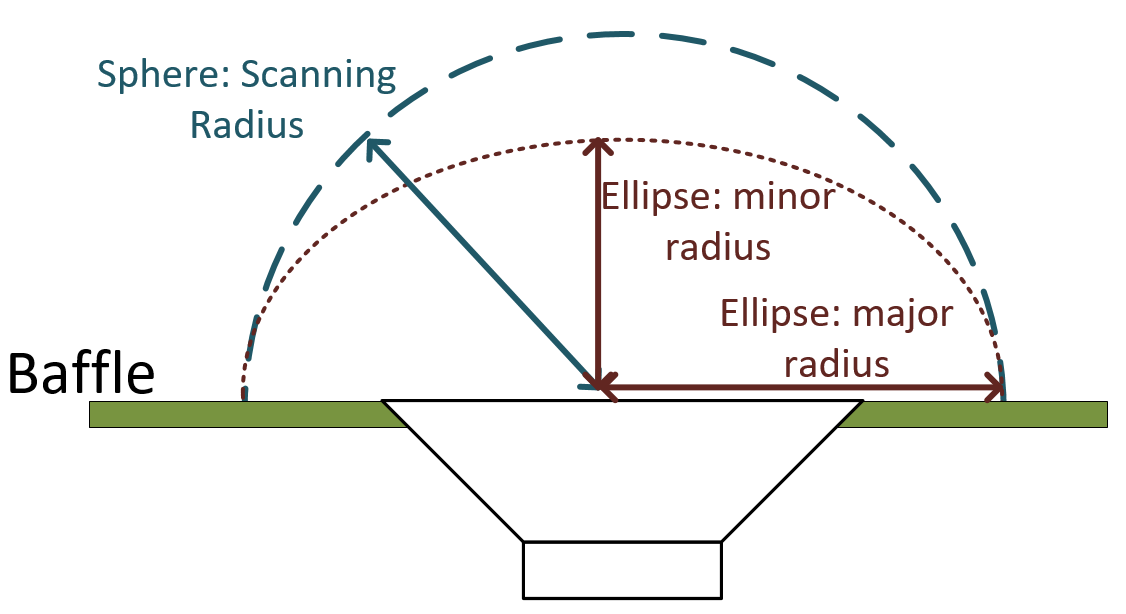
\includegraphics[scale=0.21]{GridOpti/El_Grid_Draw} 
    \captionsetup{hypcap=false} 
	\captionof{figure}{Elliptical grid} 
	\label{fig:el_grid}
\end{center}
\end{minipage}

The projection to an elliptical grid have been implemented by using the following calculations: first of all, the equation of a line $y = f(x)$ intercepting y-axis in zero gives the slope $m = \frac{y}{x}$. Introducing in the ellipse equation and using $y = m*x$ leads to a solution for x, given by equation \ref{eq:ellipse}, where a is the major radius and b the minor radius.

\begin{equation}
\left ( \frac{x}{a} \right )^{2} + \left ( \frac{y}{b} \right )^{2} = 1 \; \; \;  \Leftrightarrow \; \; \;  x = \sqrt{\frac{a^{2}b^{2}}{b^{2}+a^{2}m}}
\label{eq:ellipse}
\end{equation}
\myequations{Ellipse equation and solution for x}

The values of y-coordinates can then by calculated from the slope by using $y = mx$. 

\subsection{Measurements}

After implementation of the elliptical grid projection in Scilab, a 10cm woofer (see \ref{spkrlib:10cm}) have been measured using the NFS. The scan was performed using a spherical grid with a scanning radius of 30 cm, and an elliptical grid with a major radius of 30 cm and a minor radius of 10 cm. Both measurements have been done in the same conditions: equal input voltage, same number of points, and same position of the DUT. The results are presented in figures \ref{fig:comp_ElSPh_SPL} and \ref{fig:comp_ElSPh_Pow}. \\

\begin{minipage}{0.5\textwidth}
\begin{center}
	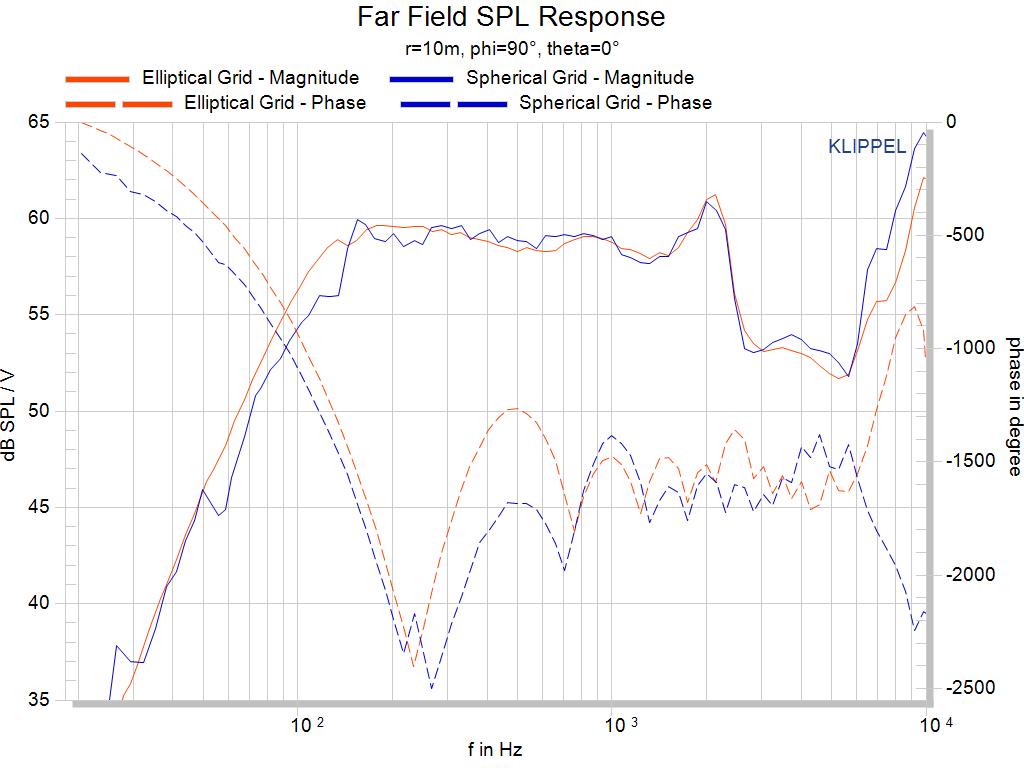
\includegraphics[width=.9\textwidth]{GridOpti/FF_Compa_El_Sph}
    \captionsetup{hypcap=false} 
	\captionof{figure}{Far Field SPL response} 
	\label{fig:comp_ElSPh_SPL}
\end{center}
\end{minipage}
\begin{minipage}{0.5\textwidth}
\begin{center}
	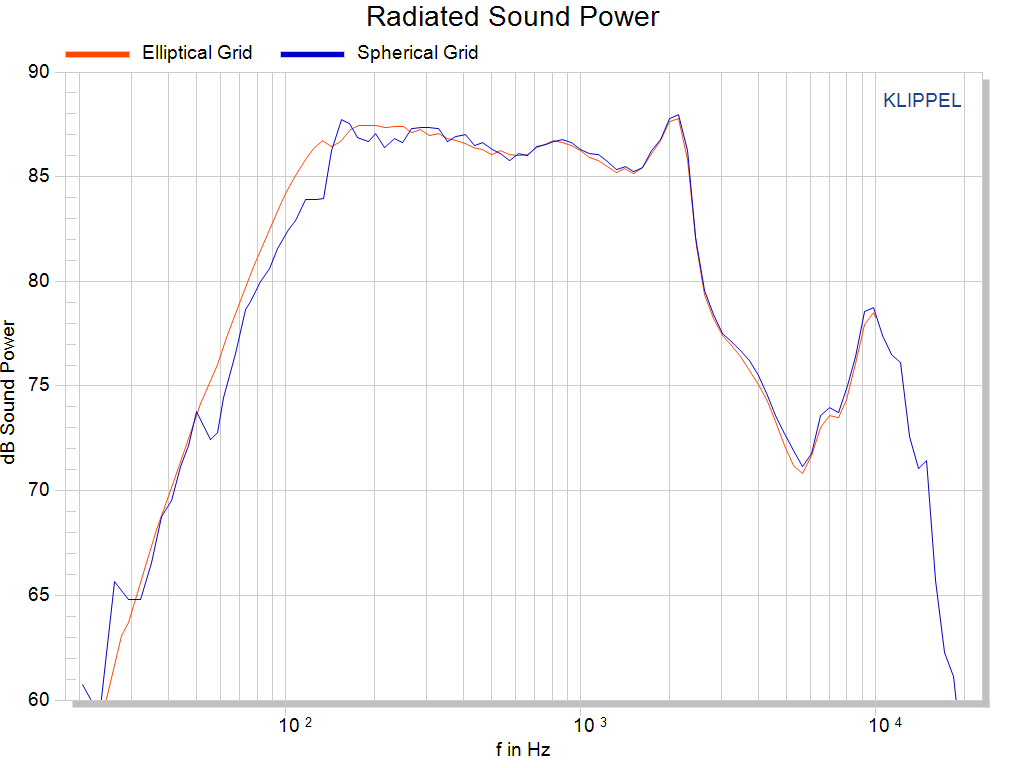
\includegraphics[width=.9\textwidth]{GridOpti/SP_Compa_El_Sph}
    \captionsetup{hypcap=false} 
	\captionof{figure}{Radiated Sound Power} 
	\label{fig:comp_ElSPh_Pow}
\end{center}
\end{minipage}
\vspace{0.1cm}

\subsection{Discussion}

Observing the magnitude of the Far Field SPL response, it can be noted that the elliptical grid provides a much smoother curve than the spherical grid, especially in the low frequencies. This effect could be explained by the fact that the measurement points being much closer to the driver, it is much less sensible to systematic errors that cannot be removed by Field Separation, such as the baffle vibrating. \\

The phase of the Far Field SPL Response gives interesting results. The elliptical grid's phase presents less phase shifts, meaning that less resonances are present on this measurement, matching with the previous hypothesis of a removed systematic error due to the baffle vibrating. \\

The radiated sound Power is extremely similar for both measurements, which was expected considering that the same speaker have been measured twice using in equal configuration. Similarly to the Far Field SPL response, the curve is smoothed when using an elliptical grid. \\

It can be concluded that using different measurement grid is relevant. A well adjusted grid have shown to give more accurate results. Following this investigation, several grids could be generated, for example a half-cylindrical grid for rectangle systems mounted in baffle, such as wall speakers.\\
Further investigations should be conducted on the influence of the measurement grid on the measurement accuracy.

% \subsection{Application note for baffle measurements}

% Another task was to create an application note to explain how to perform baffle measurements to Klippel's customers. This document being quite heavy, it is given in appendix \ref{chap:AN_Baffle}.

\section{Estimation of baffle influence}

\subsection{Presentation of the prototype}

\begin{minipage}{0.6\textwidth}
A baffle prototype have been designed to allow relevant measurements of devices mounted on a baffle with the NFS. The prototype is shown figure \ref{fig:baffle_proto}. More pictures are given in appendix \textbf{MAKE REFERENCE}. \\

Before starting the production of this item, a critical evaluation must be performed in order to estimate the influence of the baffle on the measurement. Different analysis will be conduced, mainly to check the vibration of the baffle itself, the vibration of the wood plate used to mount the speaker, and a measurement centred on the speaker in order to have a point of comparison to identify vibration problems.
\end{minipage}
\begin{minipage}{0.5\textwidth}
\begin{center}
	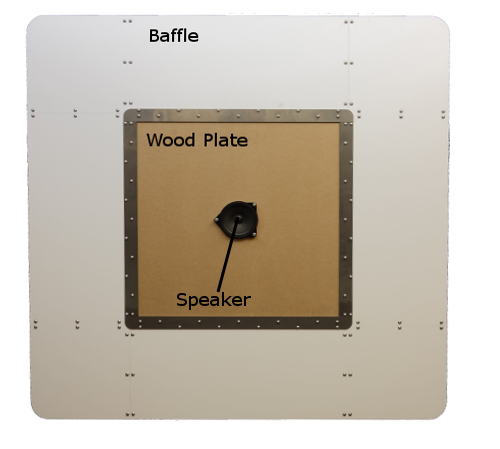
\includegraphics[scale=1.75]{GridOpti/Baffle_Alone_2} 
    \captionsetup{hypcap=false} 
	\captionof{figure}{Baffle Prototype} 
	\label{fig:baffle_proto}
\end{center}
\end{minipage} 

\subsection{Measurements}

Figure \ref{fig:vib_pow} present the apparent power in the near field of the DUT for the different measurements points. \\
The blue curve represents the power from the speaker. This scan have been centred on the speaker, using a 5cm radius for the scanning grid. The bright orange curve represents the contribution form the speaker and the wooden plate: this scan was centred on the speaker, with a 21cm radius for the scanning grid. The grey curve represents the contribution from the baffle: the scan was centred on the lower right corner of the baffle, with a 5cm scanning radius. Finally, the light orange curve represents the contribution from the wooden plate: this scan was centred midway between the speaker and the baffle, with a 5cm scanning radius. \\

Comparing the contributions from the speaker with the speaker + wood allows to estimate how the wooden plate vibration might impact the system: the differences between the 2 plots can only come from the plate vibration, as the field separation method removed all contribution from the room. \\

Comparing the variations on the speaker+wood results with the contribution of the wood shows that some of the variation matches with the peaks of the wood's contribution; whereas other matches with the baffle contribution's peaks (see figure \ref{Curves:Baffle_RadPow} for matching peaks and a bigger figure). This evaluation evidences how the baffle is polluting the measurement: the peaks observed on the SPL response could be mistaken as break-ups of the speaker.  \\

\begin{minipage}{0.5\textwidth} % Figures
\begin{center}
	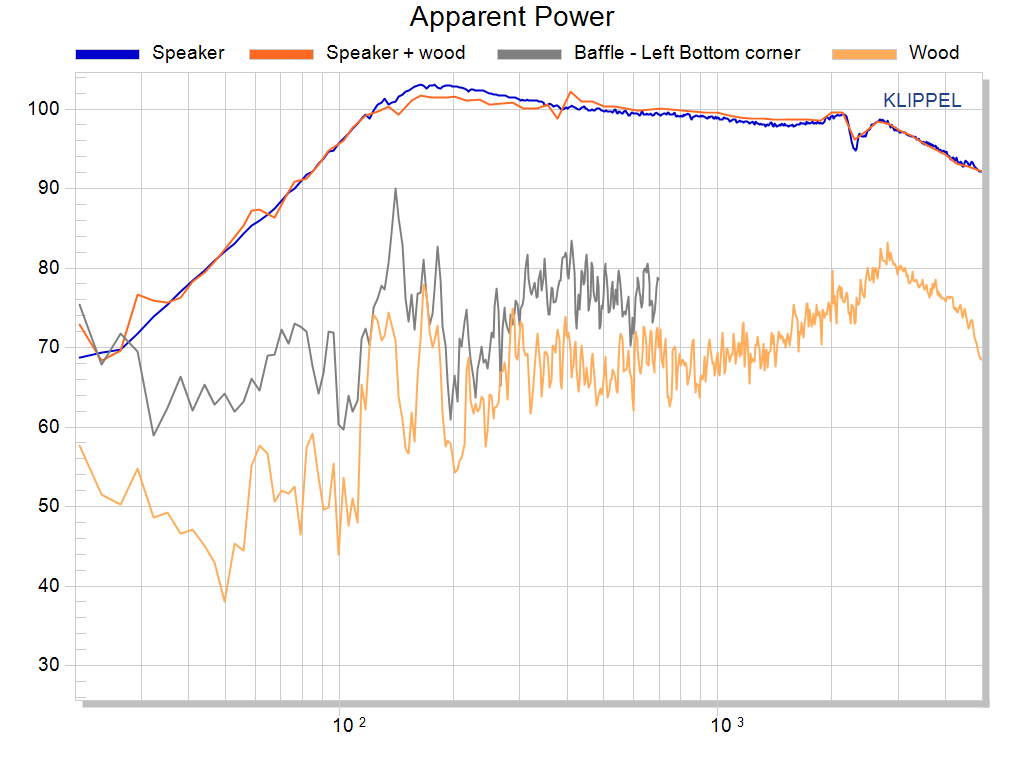
\includegraphics[width=0.9\textwidth]{GridOpti/Vib_Pow} 
\end{center}
\end{minipage}
\begin{minipage}{0.5\textwidth}
\begin{center}
	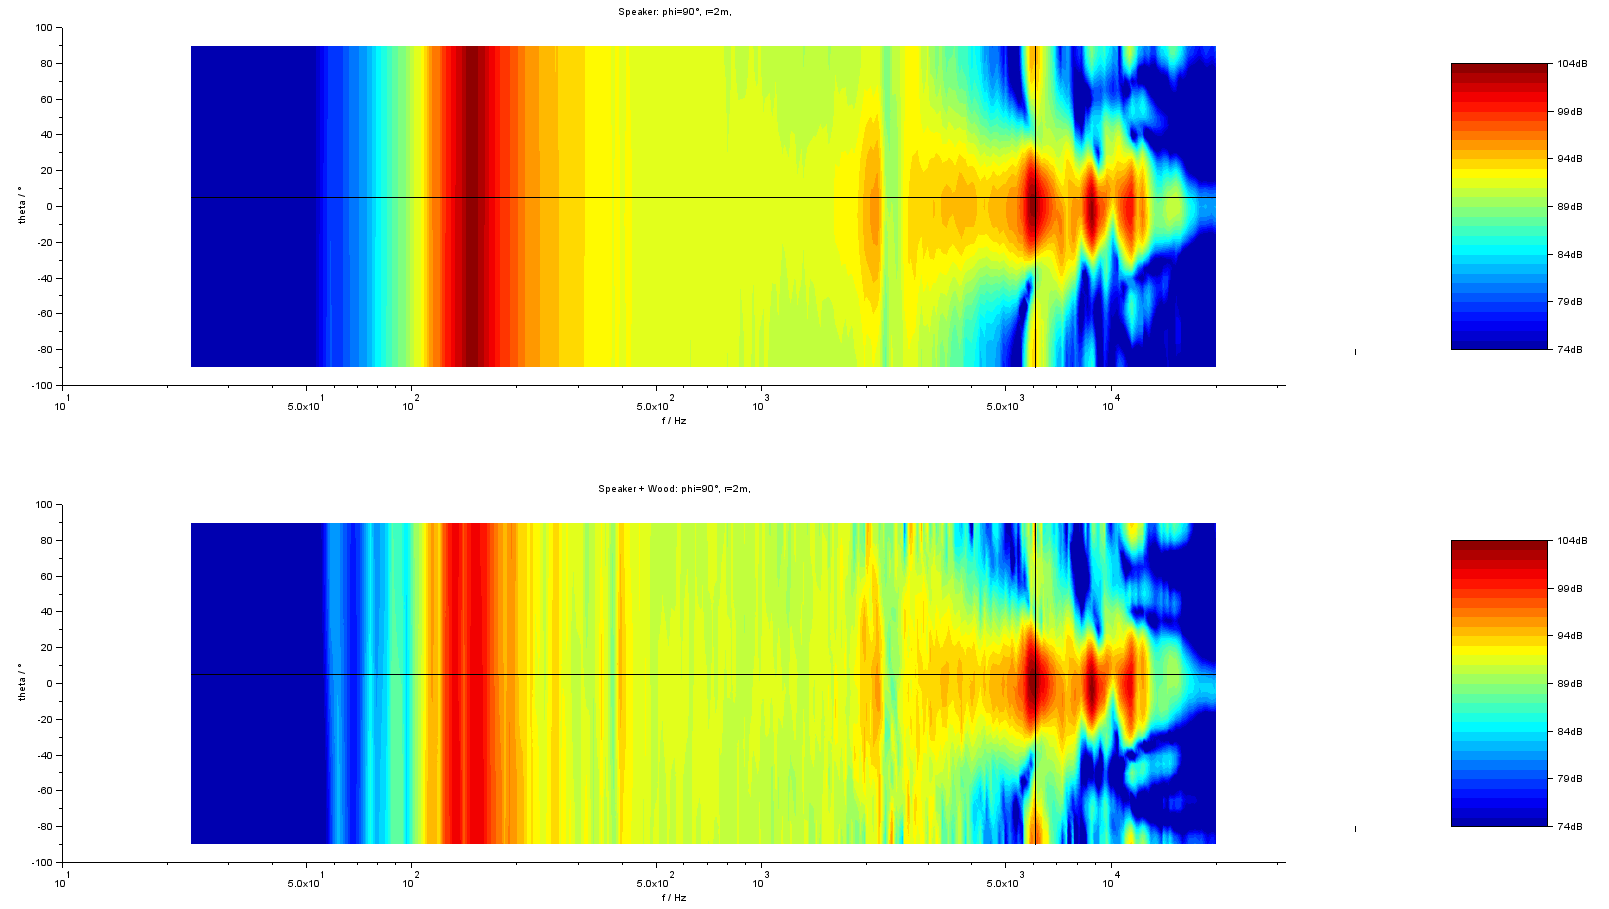
\includegraphics[width=0.9\textwidth]{GridOpti/compa_baffle_Vib} 
\end{center}
\end{minipage}

\begin{minipage}{0.5\textwidth}	% Captions of figure (2 minipages to make sure that they're aligned)
\begin{center}
    \captionsetup{hypcap=false} 
	\captionof{figure}{Comparison of apparent power in the Near Field for different measurement points} 
	\label{fig:vib_pow}
\end{center}
\end{minipage}
\begin{minipage}{0.5\textwidth}
\begin{center}
    \captionsetup{hypcap=false} 
	\captionof{figure}{Comparison of contour plots for speaker only (top) ans speaker+wood (bottom)} 
	\label{fig:vib_comp}
\end{center}
\end{minipage}\\


Figure \ref{fig:vib_comp} presents the contour plot of the speaker and the speaker+wood measurements, for a frequency range of 20Hz - 5kHz and angles from -180° to 180°. This plots are very similar, however the measurement of speaker + wood presents much more fluctuations on the side lobes and the DUT stops emitting as a monopole sooner than the speaker alone: at around 770Hz for the speaker alone, and 350Hz for the speaker + wood.\\

Figure \ref{Curves:Baffle_BalloonComp} presents a comparison of the directivity balloon at 4m and 5kHz for the speaker and the speaker + wood measurement. When observing the side lobes, it is clear that the speaker + wood configuration has more interferences than the speaker alone. This phenomenon is clearly visible on figure \ref{Curves:Baffle_BalloonWood}, which presents the directivity balloon of the speaker+wood measure at 10kHz and 10m. The contribution from the speaker is in the middle, and the side lobs shows some very strong peaks in SPL. \\
Observing the phase balloon in figure \ref{Curves:Baffle_BalloonWood} shows that the side lobes are in opposite phase with the main lobe. This observation confirms the previous hypothesis of this sides lobes being generated by the plate vibrating. 

\subsection{Discussion}

The previous investigations highlighted several problems with the baffle prototype.
\begin{itemize}
\item \textbf{Wooden plate}: special attention should be given to its thickness, material and damping. A solution to attenuate the vibration of the plate would be to stiffen it by attaching beams to the backside. As a general advice, MDF should be avoided because of its lightness. 
\item \textbf{Clamping system}: despite being very nicely engineered, the system clamping the plate in place is not satisfying to conduct acoustical measurements. The nuts supposed to hold the wooden plate in place are subject to rattling, even when strongly tightened.
\item \textbf{Baffle}: the baffle itself generates some vibration, that is believed to not be too critical for the measurements. Maybe damping could be added, although the baffle cannot be modified too much. 
\end{itemize}


%--------------------------------------------------------------
%	SYMMETRY
%--------------------------------------------------------------

\chapter{Measurement time optimization}

\section{Principle}

Exploiting symmetry conditions on the complex coefficients of the spherical wave expansion ($c_{n,m}^{out}(j \omega)$, see equation \ref{eq:sphwvexp}) could reduce the measurement time significantly by reducing the number of points of the measurement as explained in the article \textit{Holographic Nearfield Measurement of Loudspeaker Directivity} \citep[][sect.~4]{aeshs}. \\

To implement this, the idea is to start from a measurement done with a coarse grid, and to check the symmetry condition on the coefficients by using the different equations provided in appendix \ref{chap:sym}. Once the coefficients satisfying each symmetry condition have been found, the symmetry factor (given by equations \ref{eq:Srs}, \ref{eq:Sbs}, \ref{eq:Sbs}, \ref{eq:Ssps}) is estimated. By setting different thresholds, the user is informed that the DUT may present certain types of symmetry that could be used to perform a faster full measurement.

\section{Measurement on different speakers}

To verify the validity of this symmetry check, different measurements have been performed of several speakers presenting interesting geometries. A library of these speakers is given in appendix \ref{chap:spk_lib}. 

\subsection{10 cm woofer}

The DUT is a circular, 10cm woofer (see appendix \ref{spkrlib:10cm}), mounted on the baffle. \\

\begin{minipage}{0.5\textwidth}
\begin{center}
	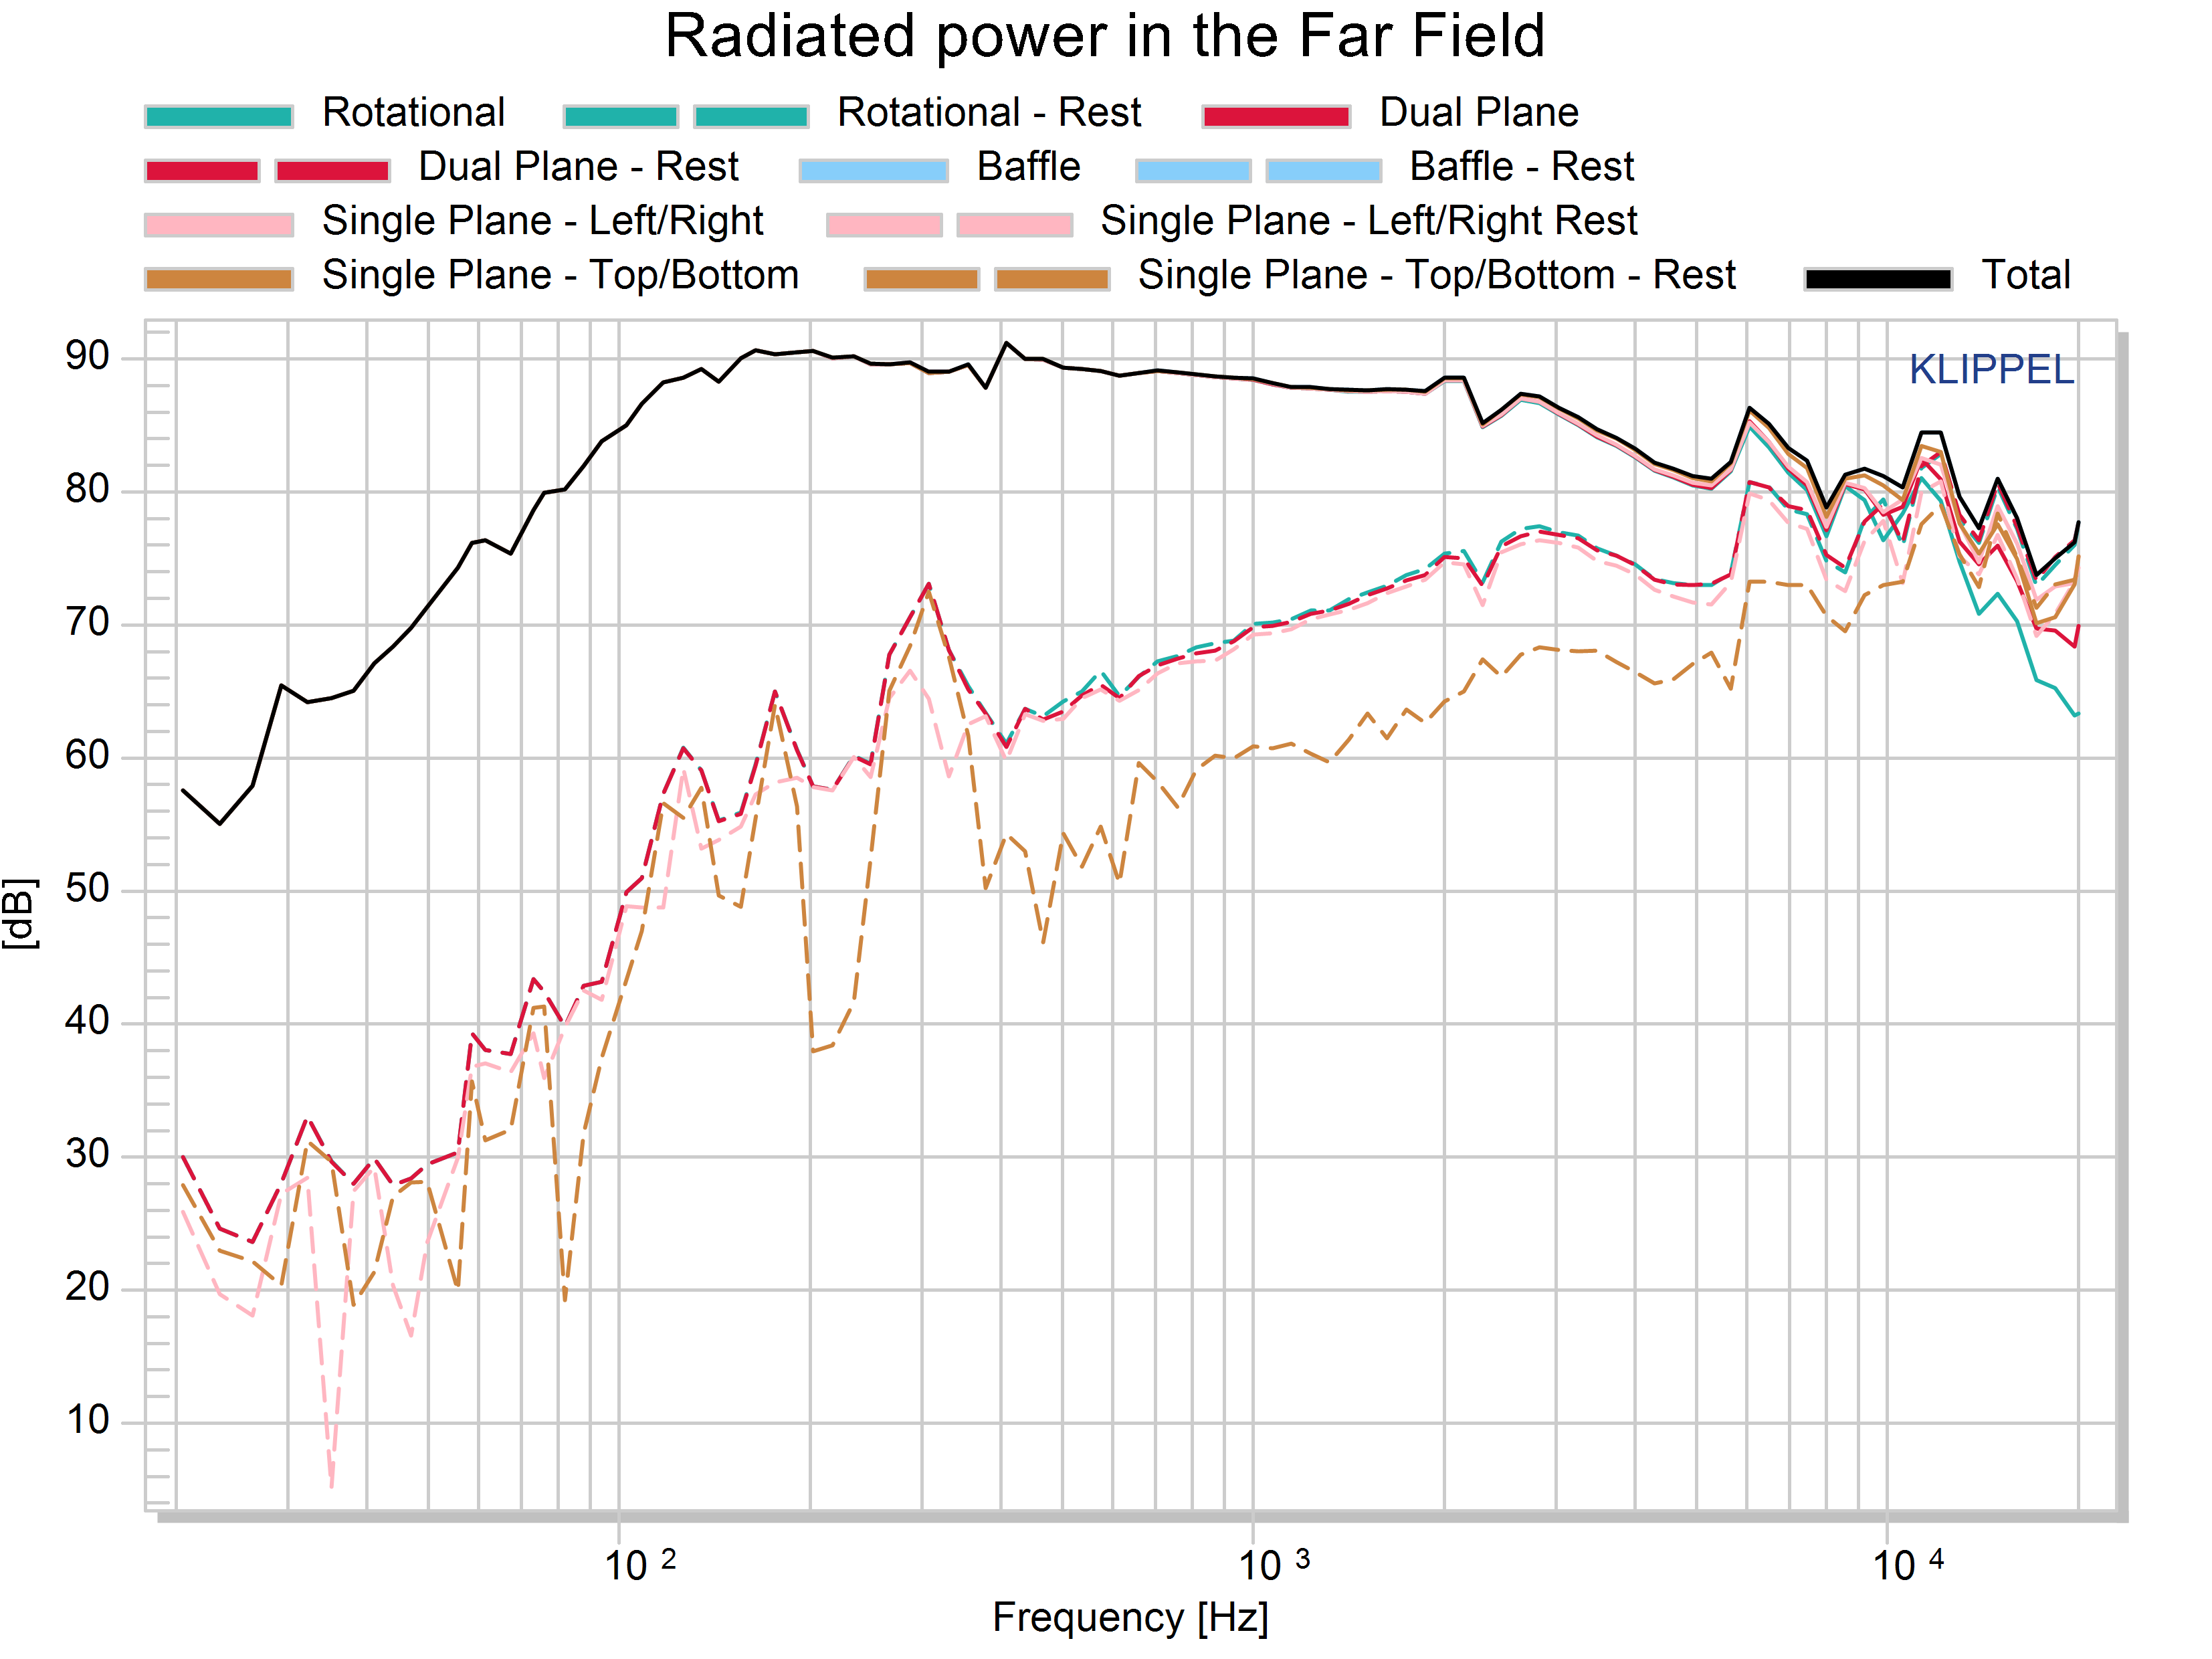
\includegraphics[width=.9\textwidth]{Sym/Rad_Pow_10cmWoofer} 
    \captionsetup{hypcap=false} 
	\captionof{figure}{Radiated Powers of 10cm woofer} 
	\label{fig:rad_pow_10cm}
\end{center}
\end{minipage}
\begin{minipage}{0.5\textwidth}
\begin{center}
	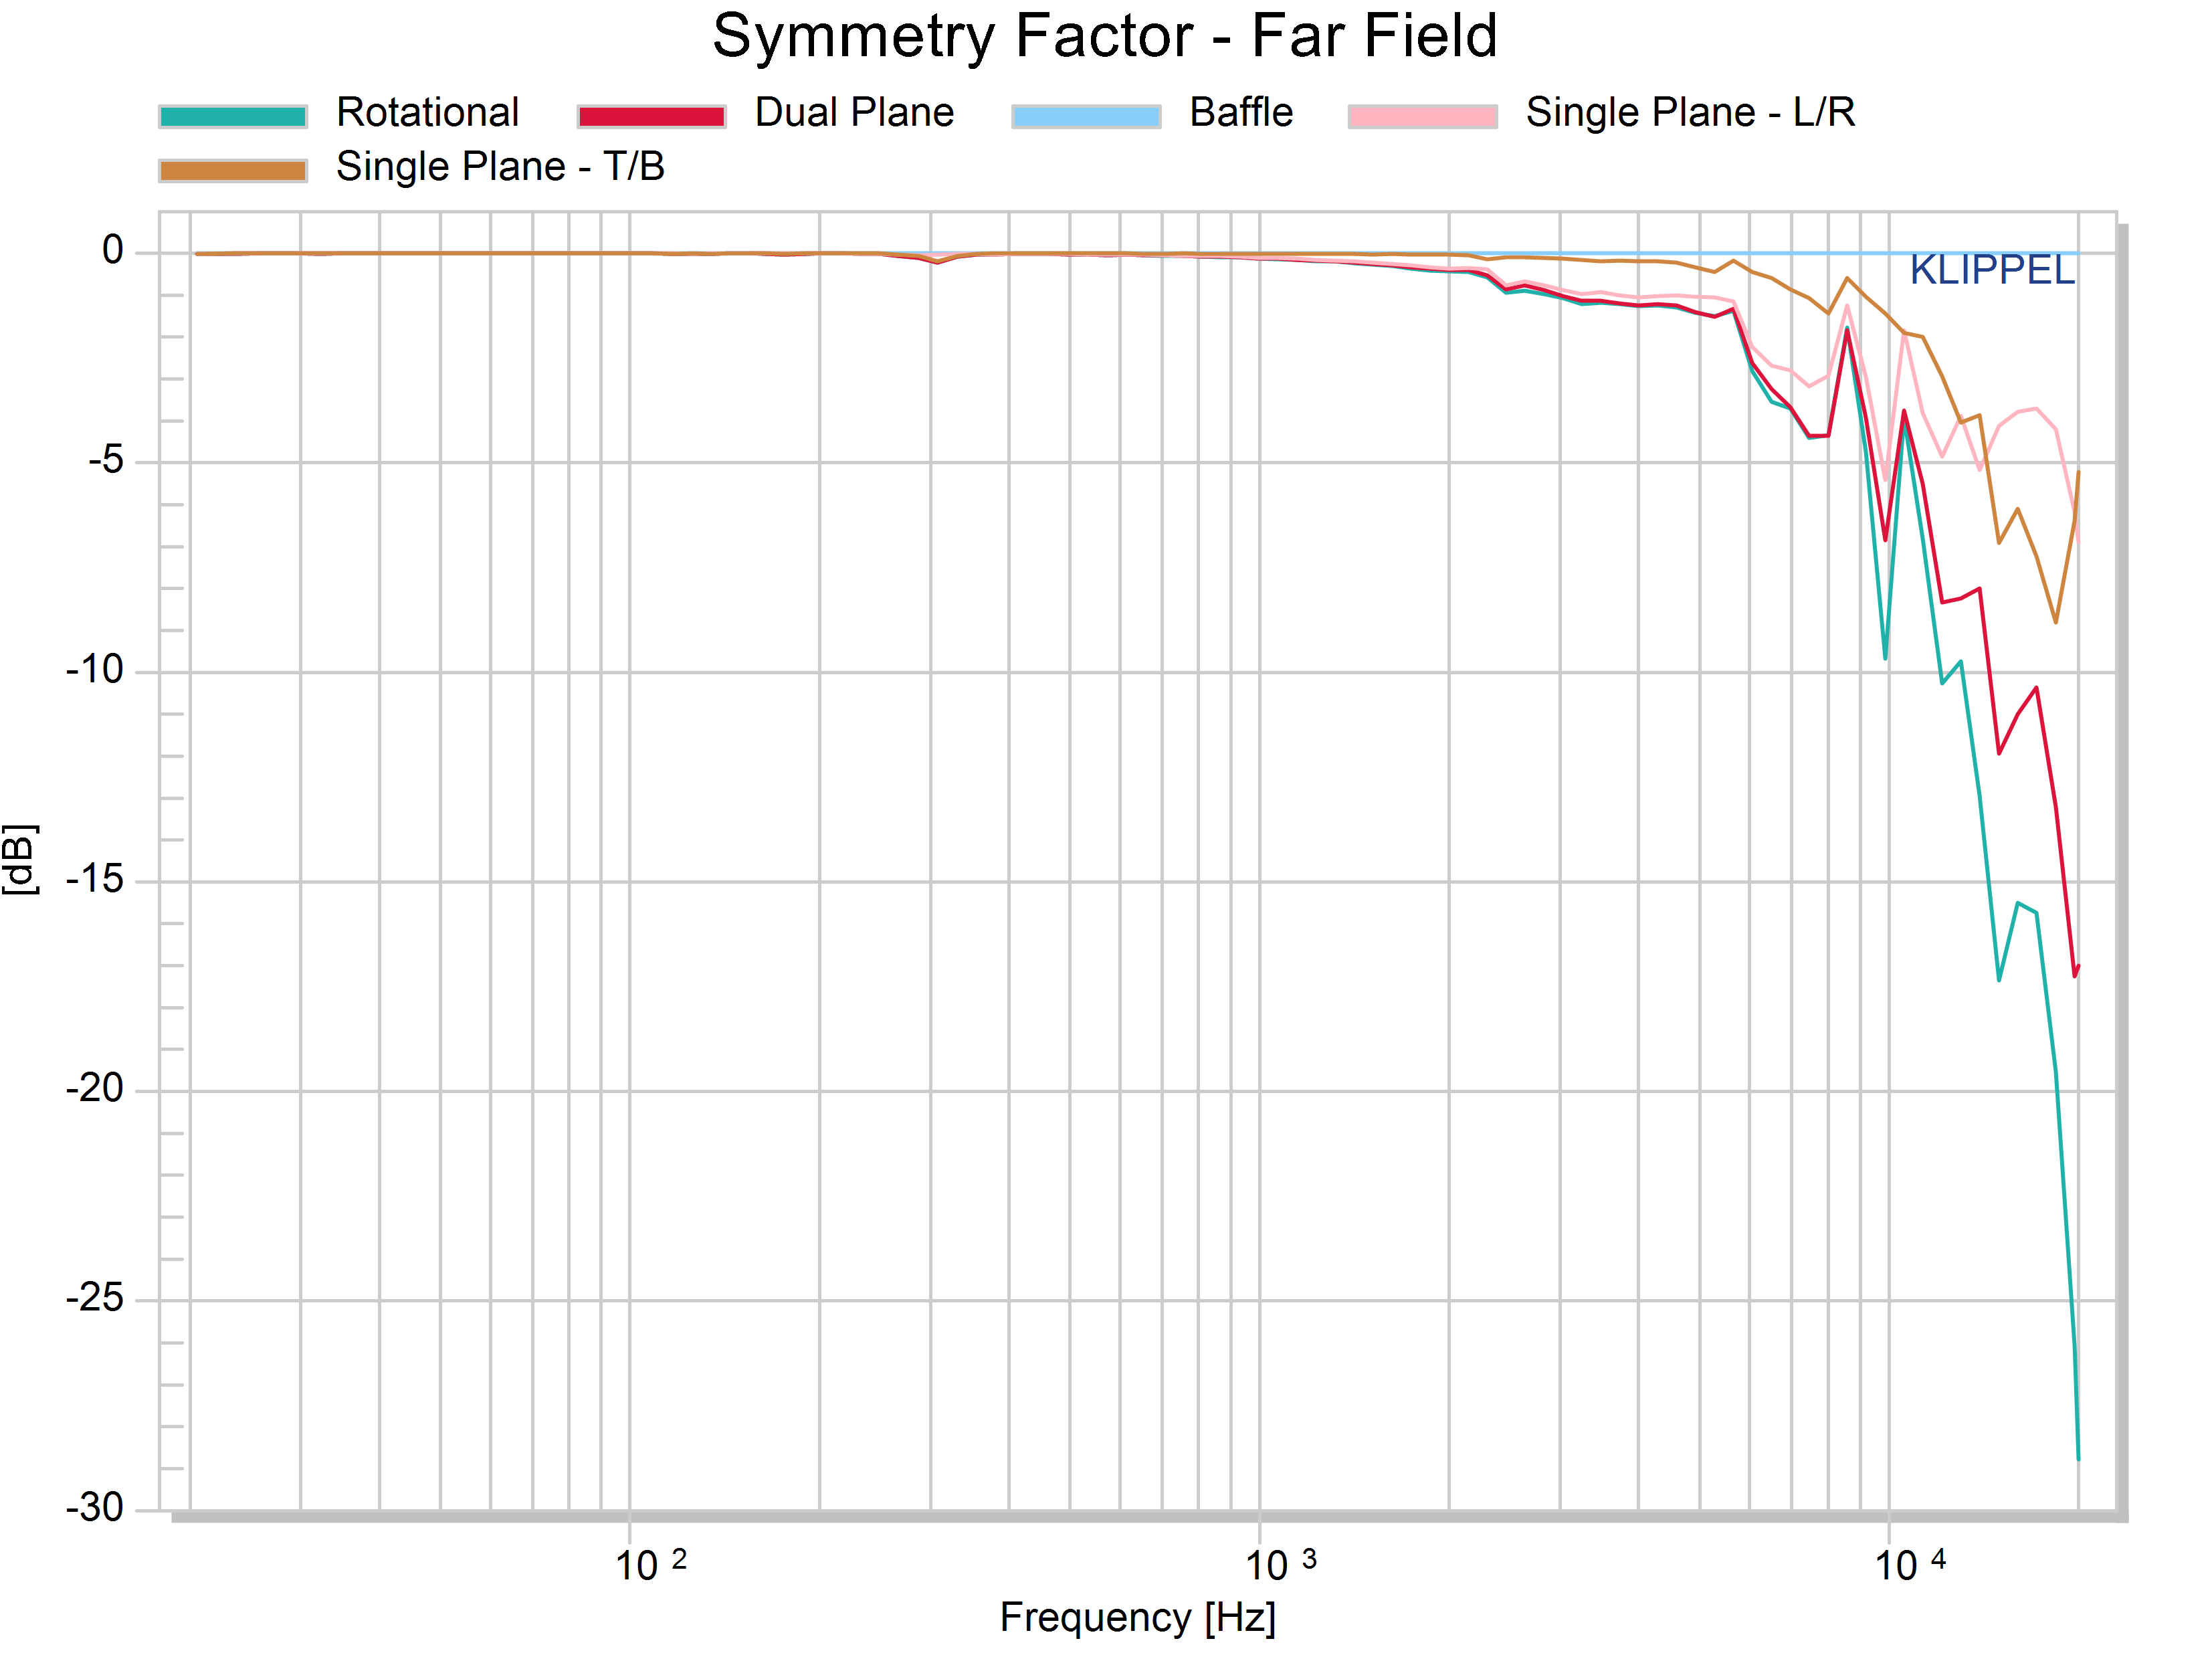
\includegraphics[width=.9\textwidth]{Sym/Sym_Fact_10cmWoofer} 
    \captionsetup{hypcap=false} 
	\captionof{figure}{Symmetry Factors of 10cm woofer} 
	\label{fig:sym_fact_10cm}
\end{center}
\end{minipage}
\vspace{0.1cm}


Figure \ref{fig:rad_pow_10cm} presents the calculated radiated powers for different symmetry conditions. The dashed curves represents the "rest", which is the radiated power for coefficients not fitting the symmetry condition (see \ref{chap:sym}, for example for a rotational symmetry the rest will be all coefficients $C_{mn} \neq 0 \;  \textup{for m}  \neq 0$). \\

Figure \ref{fig:sym_fact_10cm} presents the symmetry factors for different types of symmetry, in dB. A 0 dB value means that the different between the radiated power of the symmetry condition and the radiated powers of the rest presents no difference. Observing the symmetry factor for the baffle shows that this value is constantly 0 on the whole frequency band: this result is matching the expectation since the measurement have been done with the speaker mounted on a baffle. \\

Comparing the radiated power in figure \ref{fig:rad_pow_10cm} for the different symmetries gives interesting results: in the low frequency domain, the total radiated power and different powers are extremely similar, no matter the symmetry type. In high frequencies, disruptions appears and the rest increases significantly: the higher the frequency, and the more interferences will be produced by the speaker. \\

Comparing the symmetry factor shows that the most present symmetries are the Single Plane symmetries. This result could be a bit surprising as the rotational symmetry is expected to be dominant, but in high frequencies the speaker does not behave as a piston: the cone breakups spoils the rotational symmetry. 

\subsection{Oval speaker}
The DUT is an oval speaker (see appendix \ref{spkrlib:oval}), mounted on the baffle. The particular geometry of this speaker gives hints about the type of symmetry that should be expected: the rotational symmetry should be the lowest one, and the plane symmetries should be dominant.  Figures \ref{fig:rad_pow_Oval} and \ref{fig:sym_fact_Oval} presents the radiated powers and the symmetry factors respectively.\\

\begin{minipage}{0.5\textwidth}
\begin{center}
	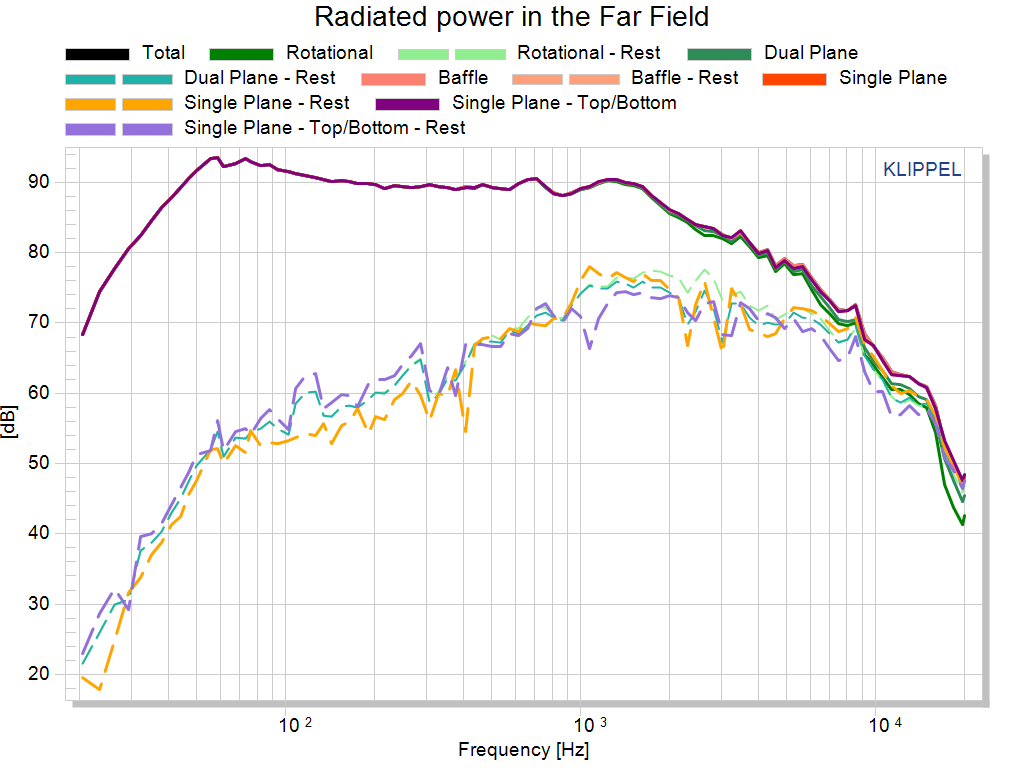
\includegraphics[width=.9\textwidth]{Sym/Rad_Pow_OvalSpkr} 
    \captionsetup{hypcap=false} 
	\captionof{figure}{Radiated Powers of oval speaker} 
	\label{fig:rad_pow_Oval}
\end{center}
\end{minipage}
\begin{minipage}{0.5\textwidth}
\begin{center}
	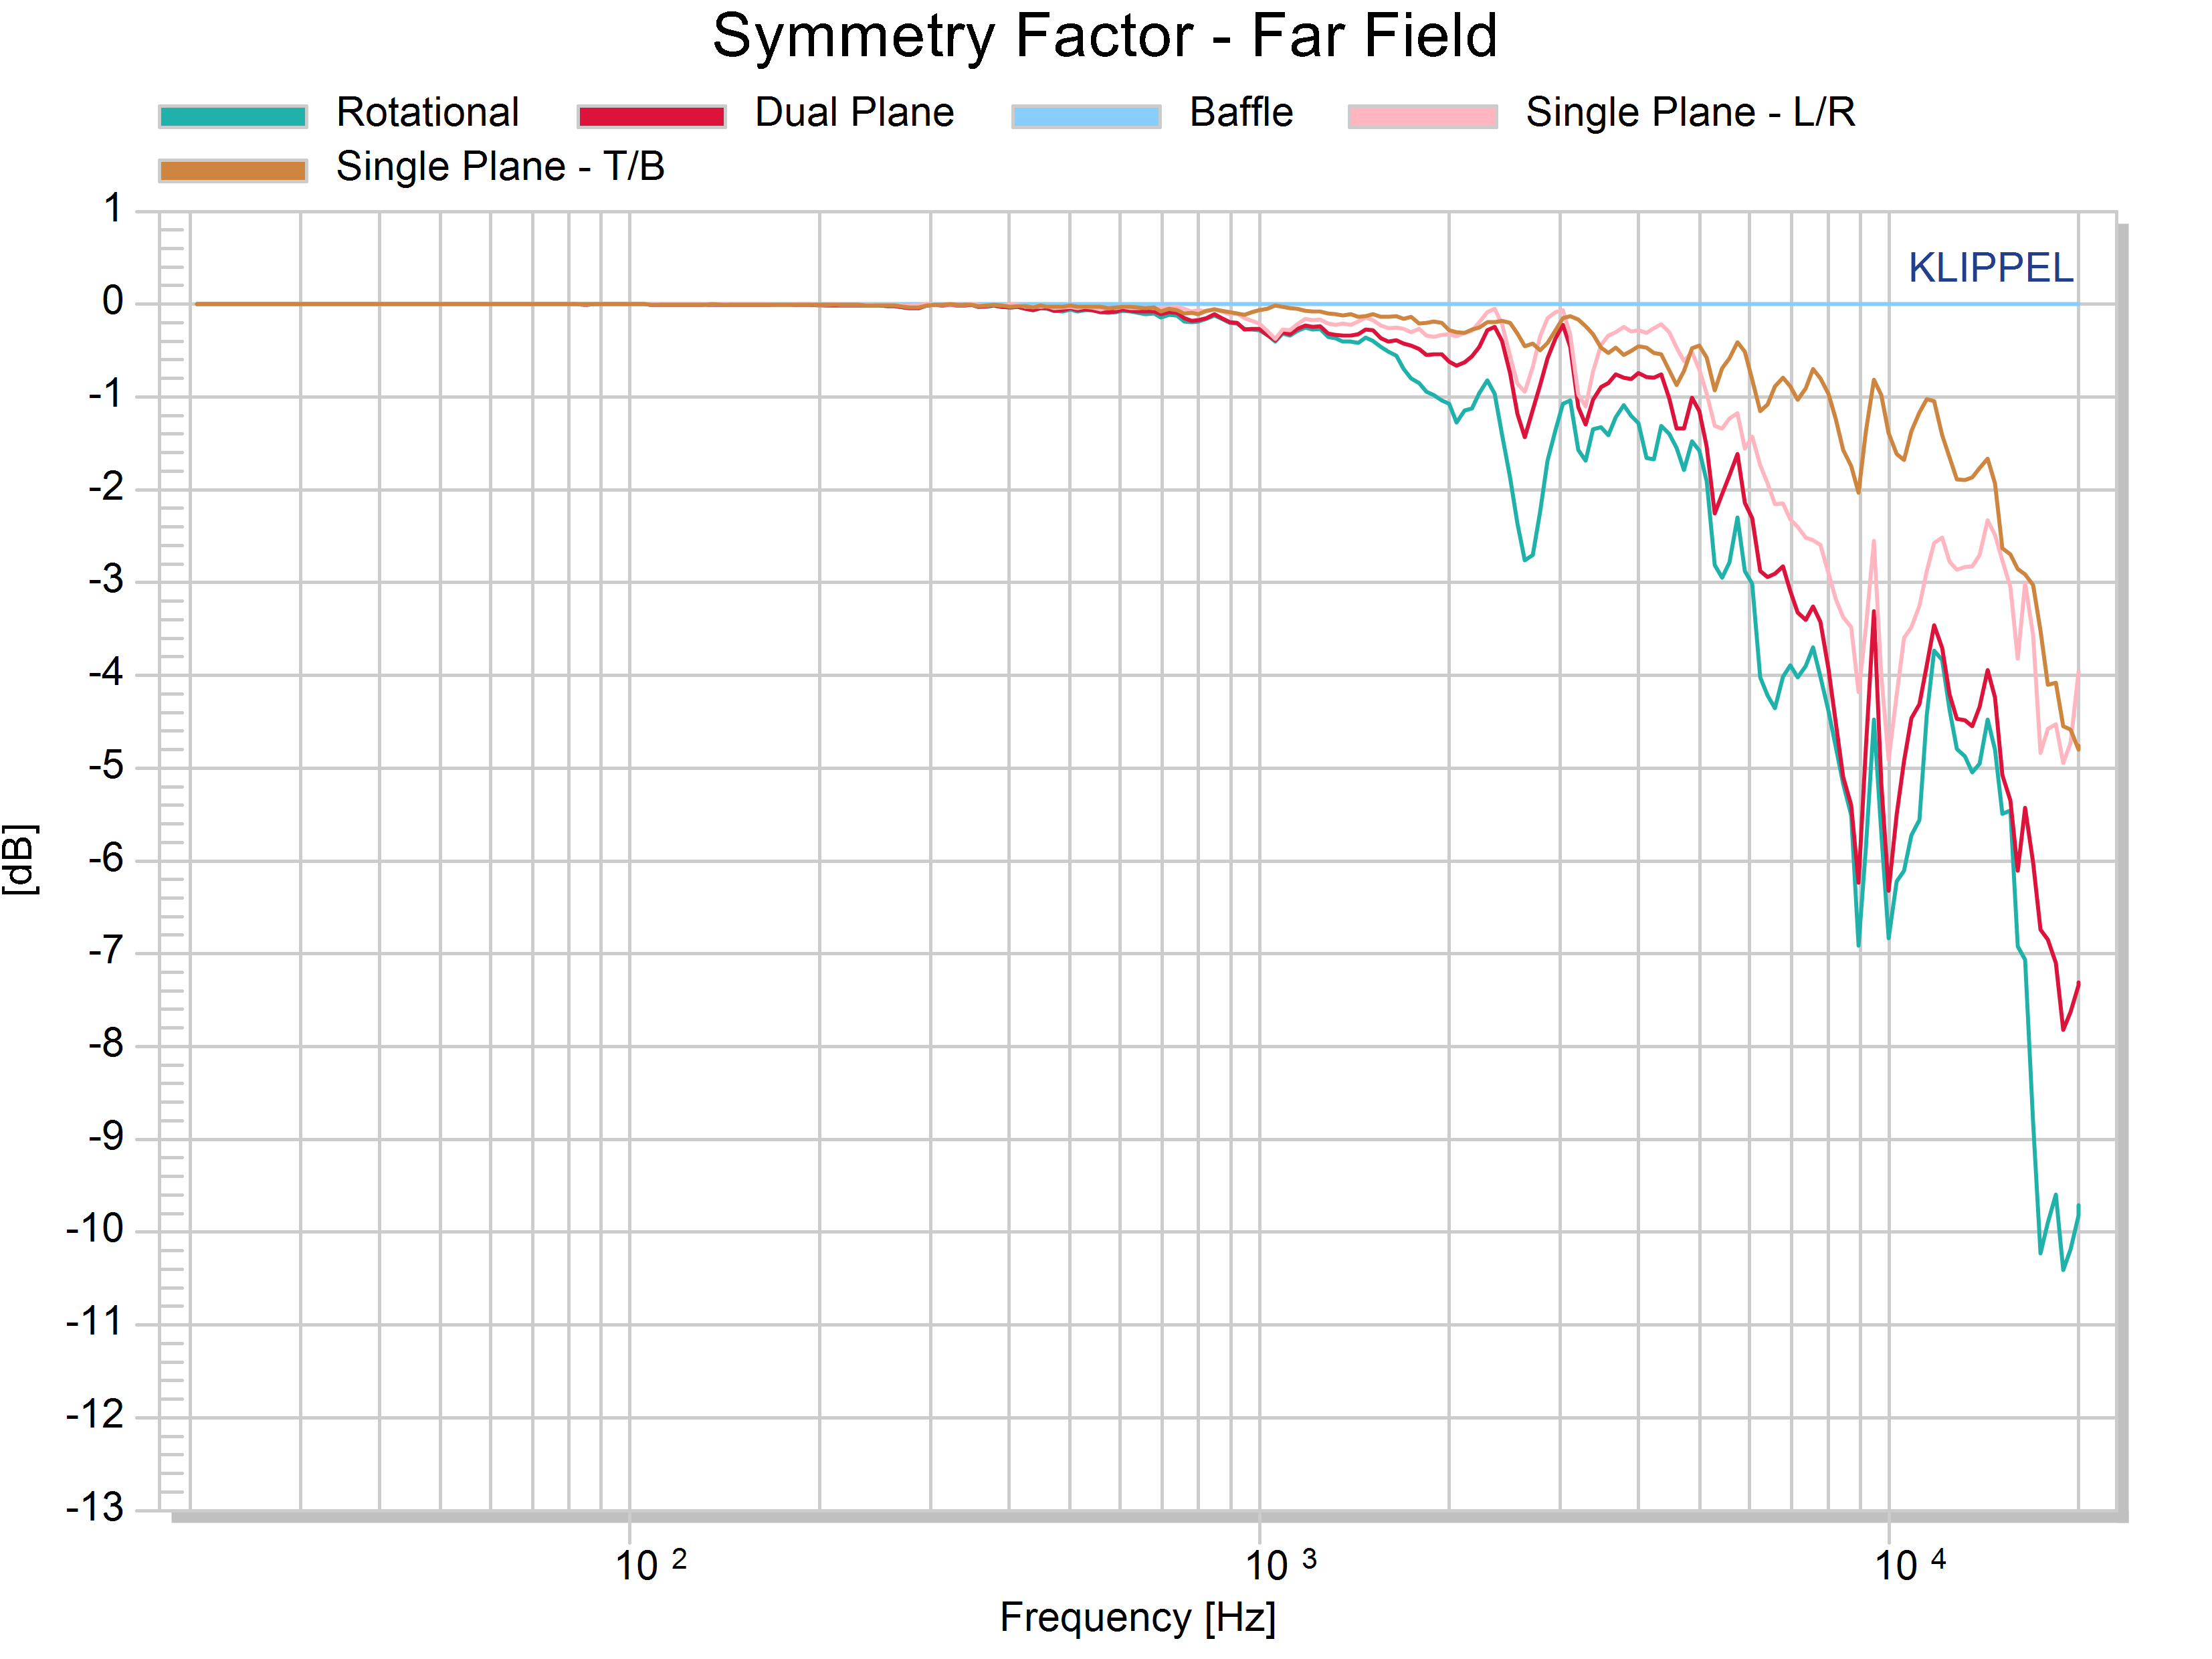
\includegraphics[width=.9\textwidth]{Sym/Sym_Fact_OvalSpkr} 
    \captionsetup{hypcap=false} 
	\captionof{figure}{Symmetry Factors of oval speaker} 
	\label{fig:sym_fact_Oval}
\end{center}
\end{minipage}
\vspace{0.1cm}

Observing the Radiated Powers shows that expected results have been encountered: in the high frequencies (a zoom on the 7 - 20 kHz range is given in appendix \ref{Curves:oval}) from 8.5 kHz, the rest of the rotational symmetry radiated power is higher that the radiated power by the rotational symmetry. This means that there is more power given by the coefficients which do not respect the condition for rotational symmetry, than by the coefficients validating $C_{mn} = 0 \;  \textup{for m}  \neq 0$.  \\

Interestingly, the top/bottom Single Plane Symmetry factor is higher than other symmetries from 5 kHz. This could be explained by the speaker's geometry: the larger dimension makes it more prone to rocking mode, spoiling the Left/Right Single Plane Symmetry. \\
As expected, the rotational symmetry factor is below all other factors, a phenomenon that has already been observed on the Radiated Powers. 

% Make a measure with speaker shifted by 90° and compare the symmetry factors.



\subsection{2-way "diagonal" speaker}

The DUT is a "diagonal" 2-way speaker, and the scan is centred on the tweeter (see appendix \ref{spkrlib:BnO}). This speaker's asymmetrical geometry is very interesting to test the symmetry check. The device also have an integrated crossover. Figures \ref{fig:rad_pow_BnO} and \ref{fig:sym_fact_BnO} presents the radiated powers and the symmetry factors respectively. \\

The crossover frequency range can be observed clearly on both result result curves: the symmetry factors take a dip, and the rest powers are higher than the symmetrical powers (a zoom on the crossover range for the radiated powers in provided in \ref{Curves:2way}).\\

Observing the Symmetry Factors shows that there is no baffle symmetry for this measurement. Although this result might seem quite trivial since the DUT was not mounted on a baffle, it is good indication that the symmetry estimation works correctly. Another interesting observation is at the crossover frequency: the symmetry factors take a dip. \\
In this frequency range, both drivers of the DUT are working, and due to their positioning there is no possible symmetry condition. In low frequency, the driver is a monopole, so all symmetry conditions are fulfilled.\\

In high frequency when the twitter alone is emitting, some symmetry is observed. The Top/Bottom single plane symmetry have the highest coefficients, meaning that it could be possible to measure only the top half of this driver and to deduce the coefficients using equation \ref{eq:spsym}.\\

\begin{minipage}{0.5\textwidth}
\begin{center}
	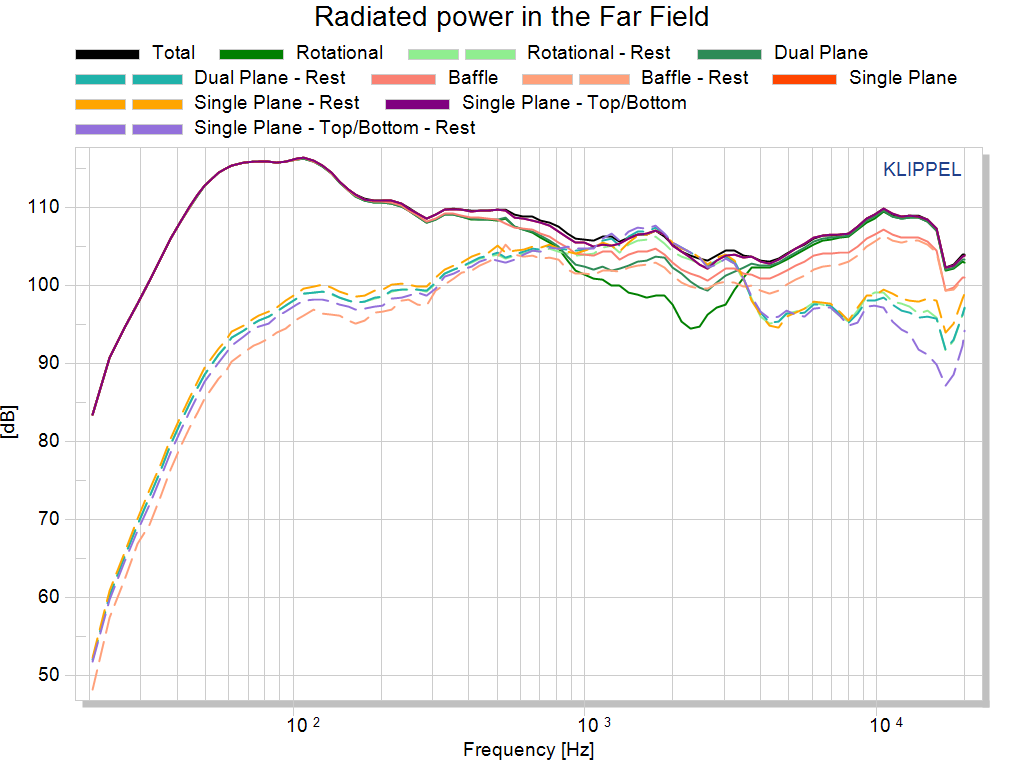
\includegraphics[width=.9\textwidth]{Sym/Rad_Pow_BnO} 
    \captionsetup{hypcap=false} 
	\captionof{figure}{Radiated Powers of diagonal speaker} 
	\label{fig:rad_pow_BnO}
\end{center}
\end{minipage}
\begin{minipage}{0.5\textwidth}
\begin{center}
	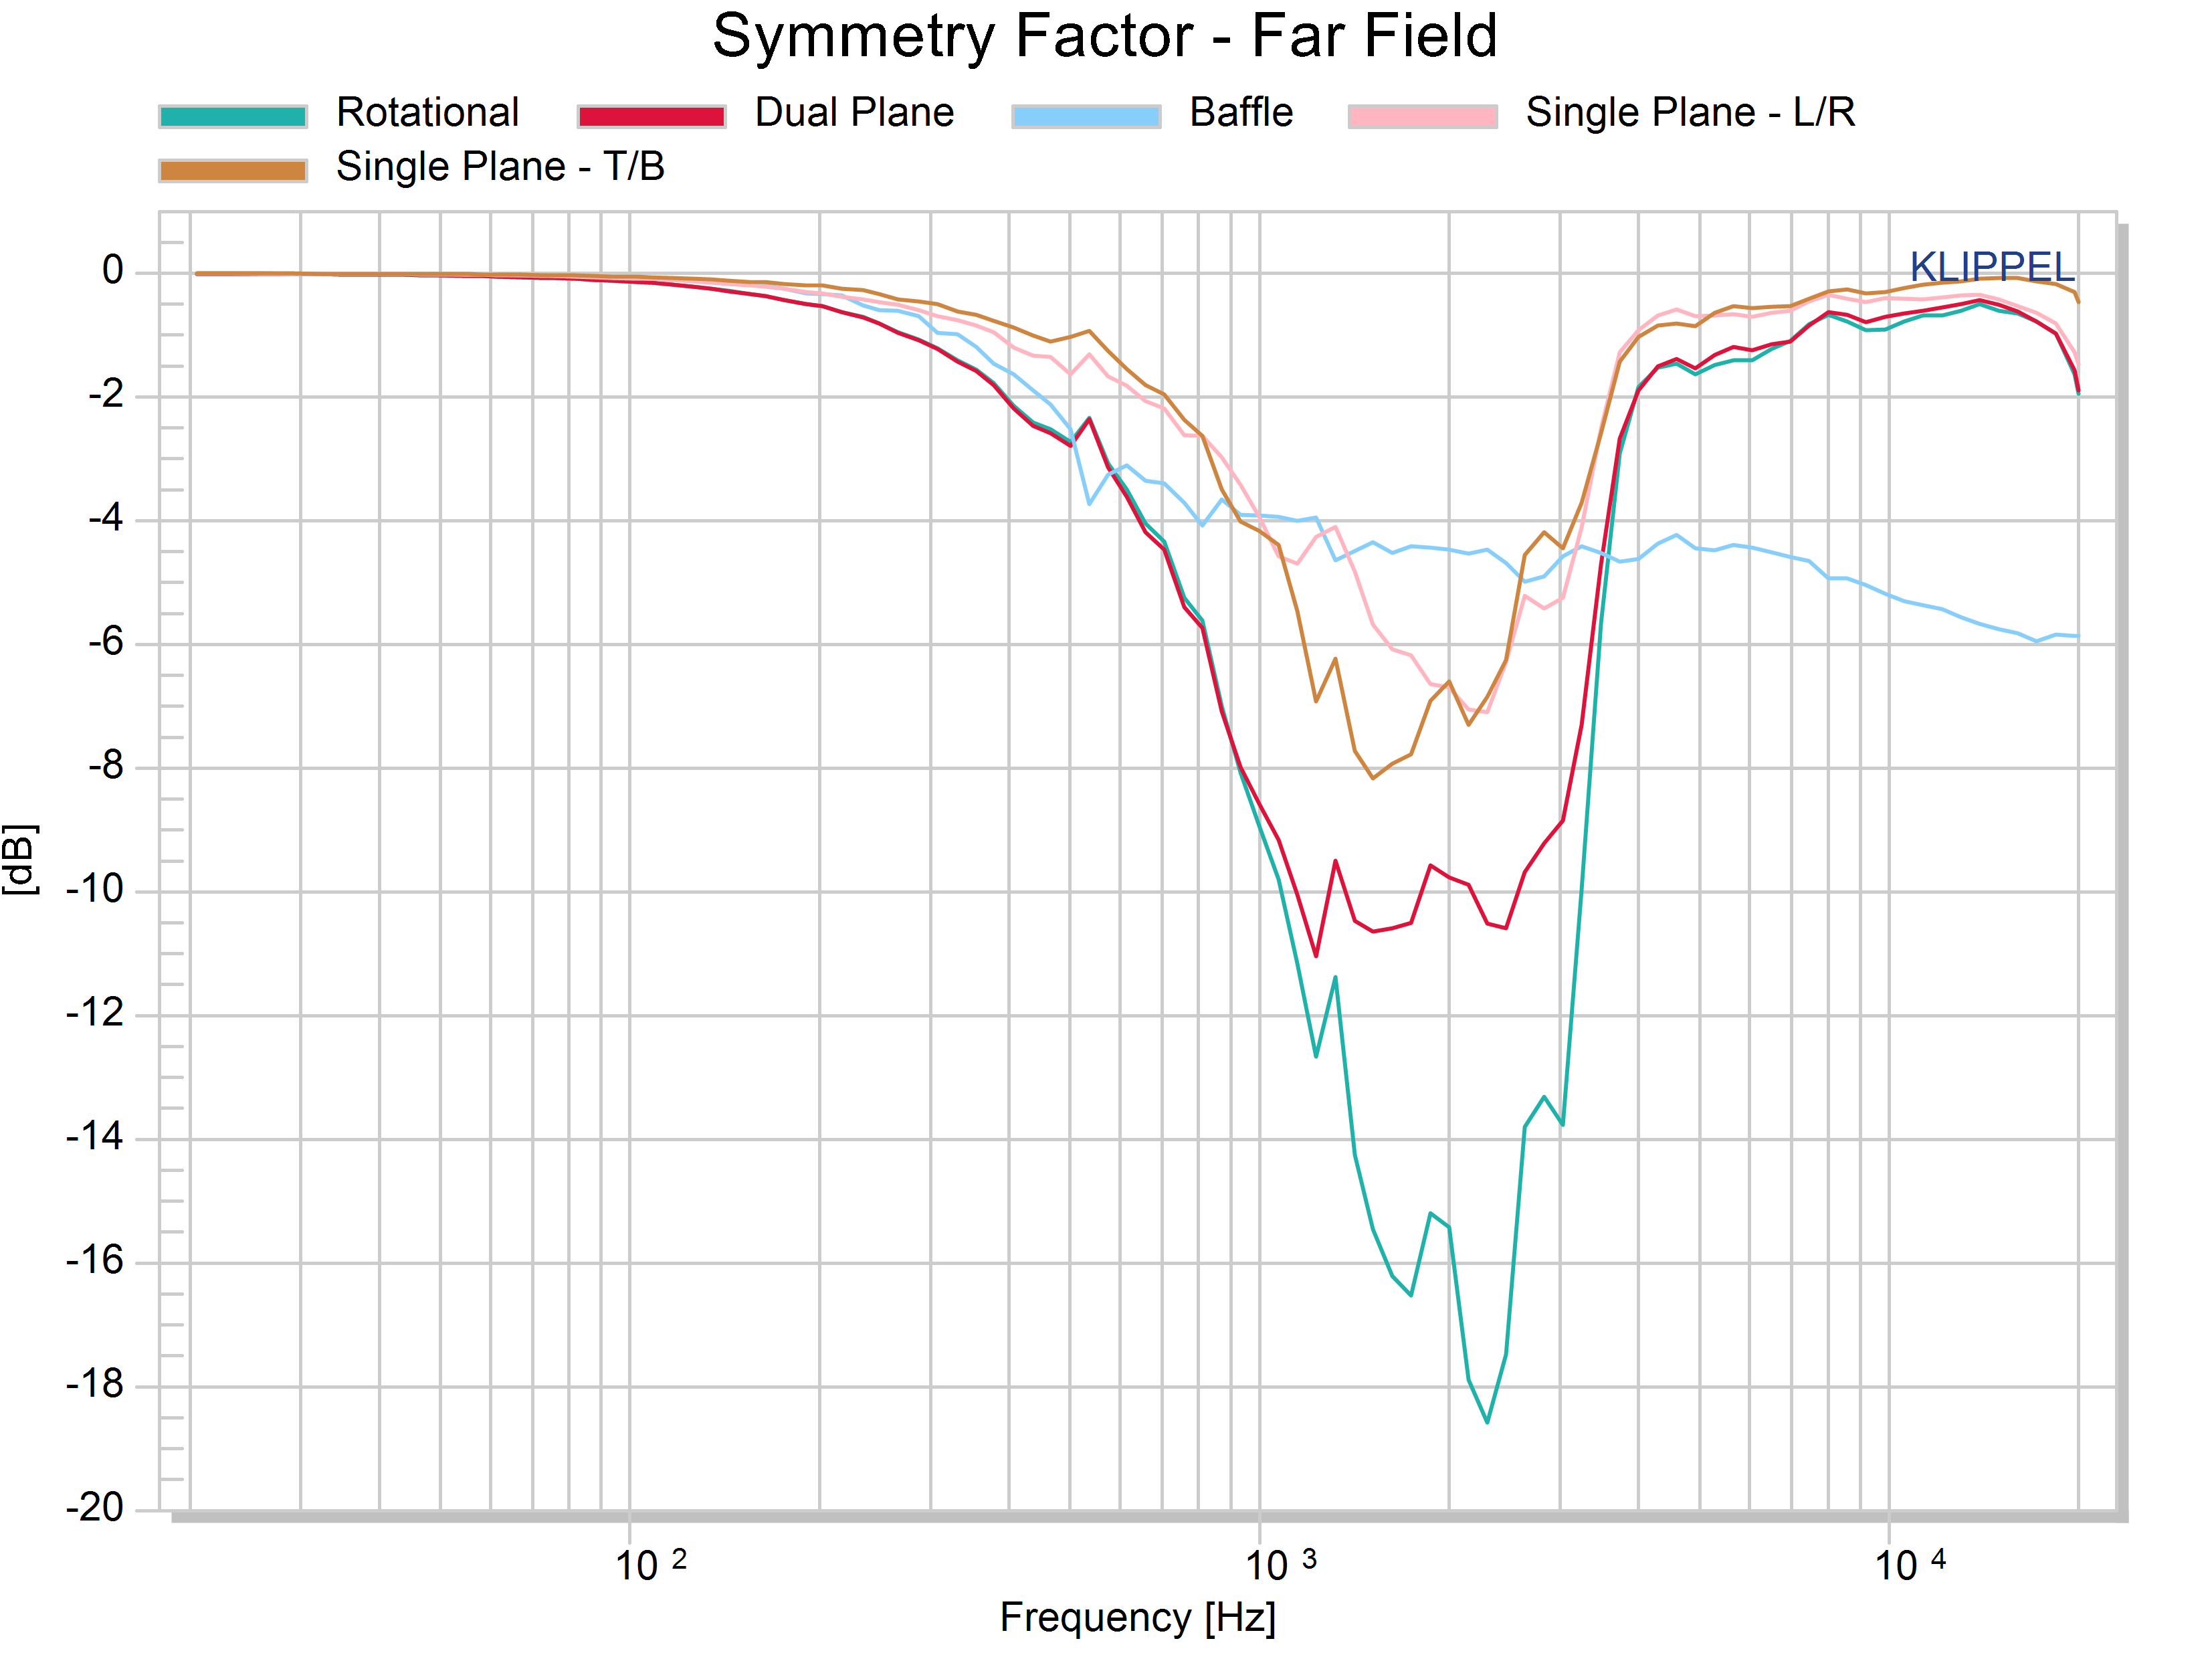
\includegraphics[width=.9\textwidth]{Sym/Sym_Fact_BnO} 
    \captionsetup{hypcap=false} 
	\captionof{figure}{Symmetry Factors of diagonal speaker} 
	\label{fig:sym_fact_BnO}
\end{center}
\end{minipage}
\vspace{0.1cm}

\section{Discussion}

The previous results are promising for the investigation on symmetry conditions to ease off the measurement time. The calculated symmetry factors match with the expected results for all measurements, and can be implemented in the NFS scripts to be exploited for reducing the number of measurements points. \\
This investigation raises several questions: 
\begin{itemize}
	\item What is the influence of the position of the speaker?
	\item Can a mispositioned DUT be detected and adjusted?
\end{itemize}

%--------------------------------------------------------------
%	ROOM CORRECTION
%--------------------------------------------------------------
\chapter{Room correction}

\section{Principle}

Being able to generate room correction curves is great for the everyday measurement of loudspeakers since it allows to compensate the effect of any environment and to create quasi-perfect measurements. According to the AES standard \cite{aesstandart}, "\textit{accurate and repeatable loudspeaker driver measurements require that environmental and boundary influence have minimal impact on the measurement}". Such measurements are usually done in anechoic rooms, and accurate results are difficult to achieve for companies not having access to such a room or for a hobbyist. \\
By using post-processing, it is possible to generate room correction curves. Several methods are available \citep[see][]{aeswb}.\\

\begin{minipage}{0.33333333\textwidth}
\begin{center}
	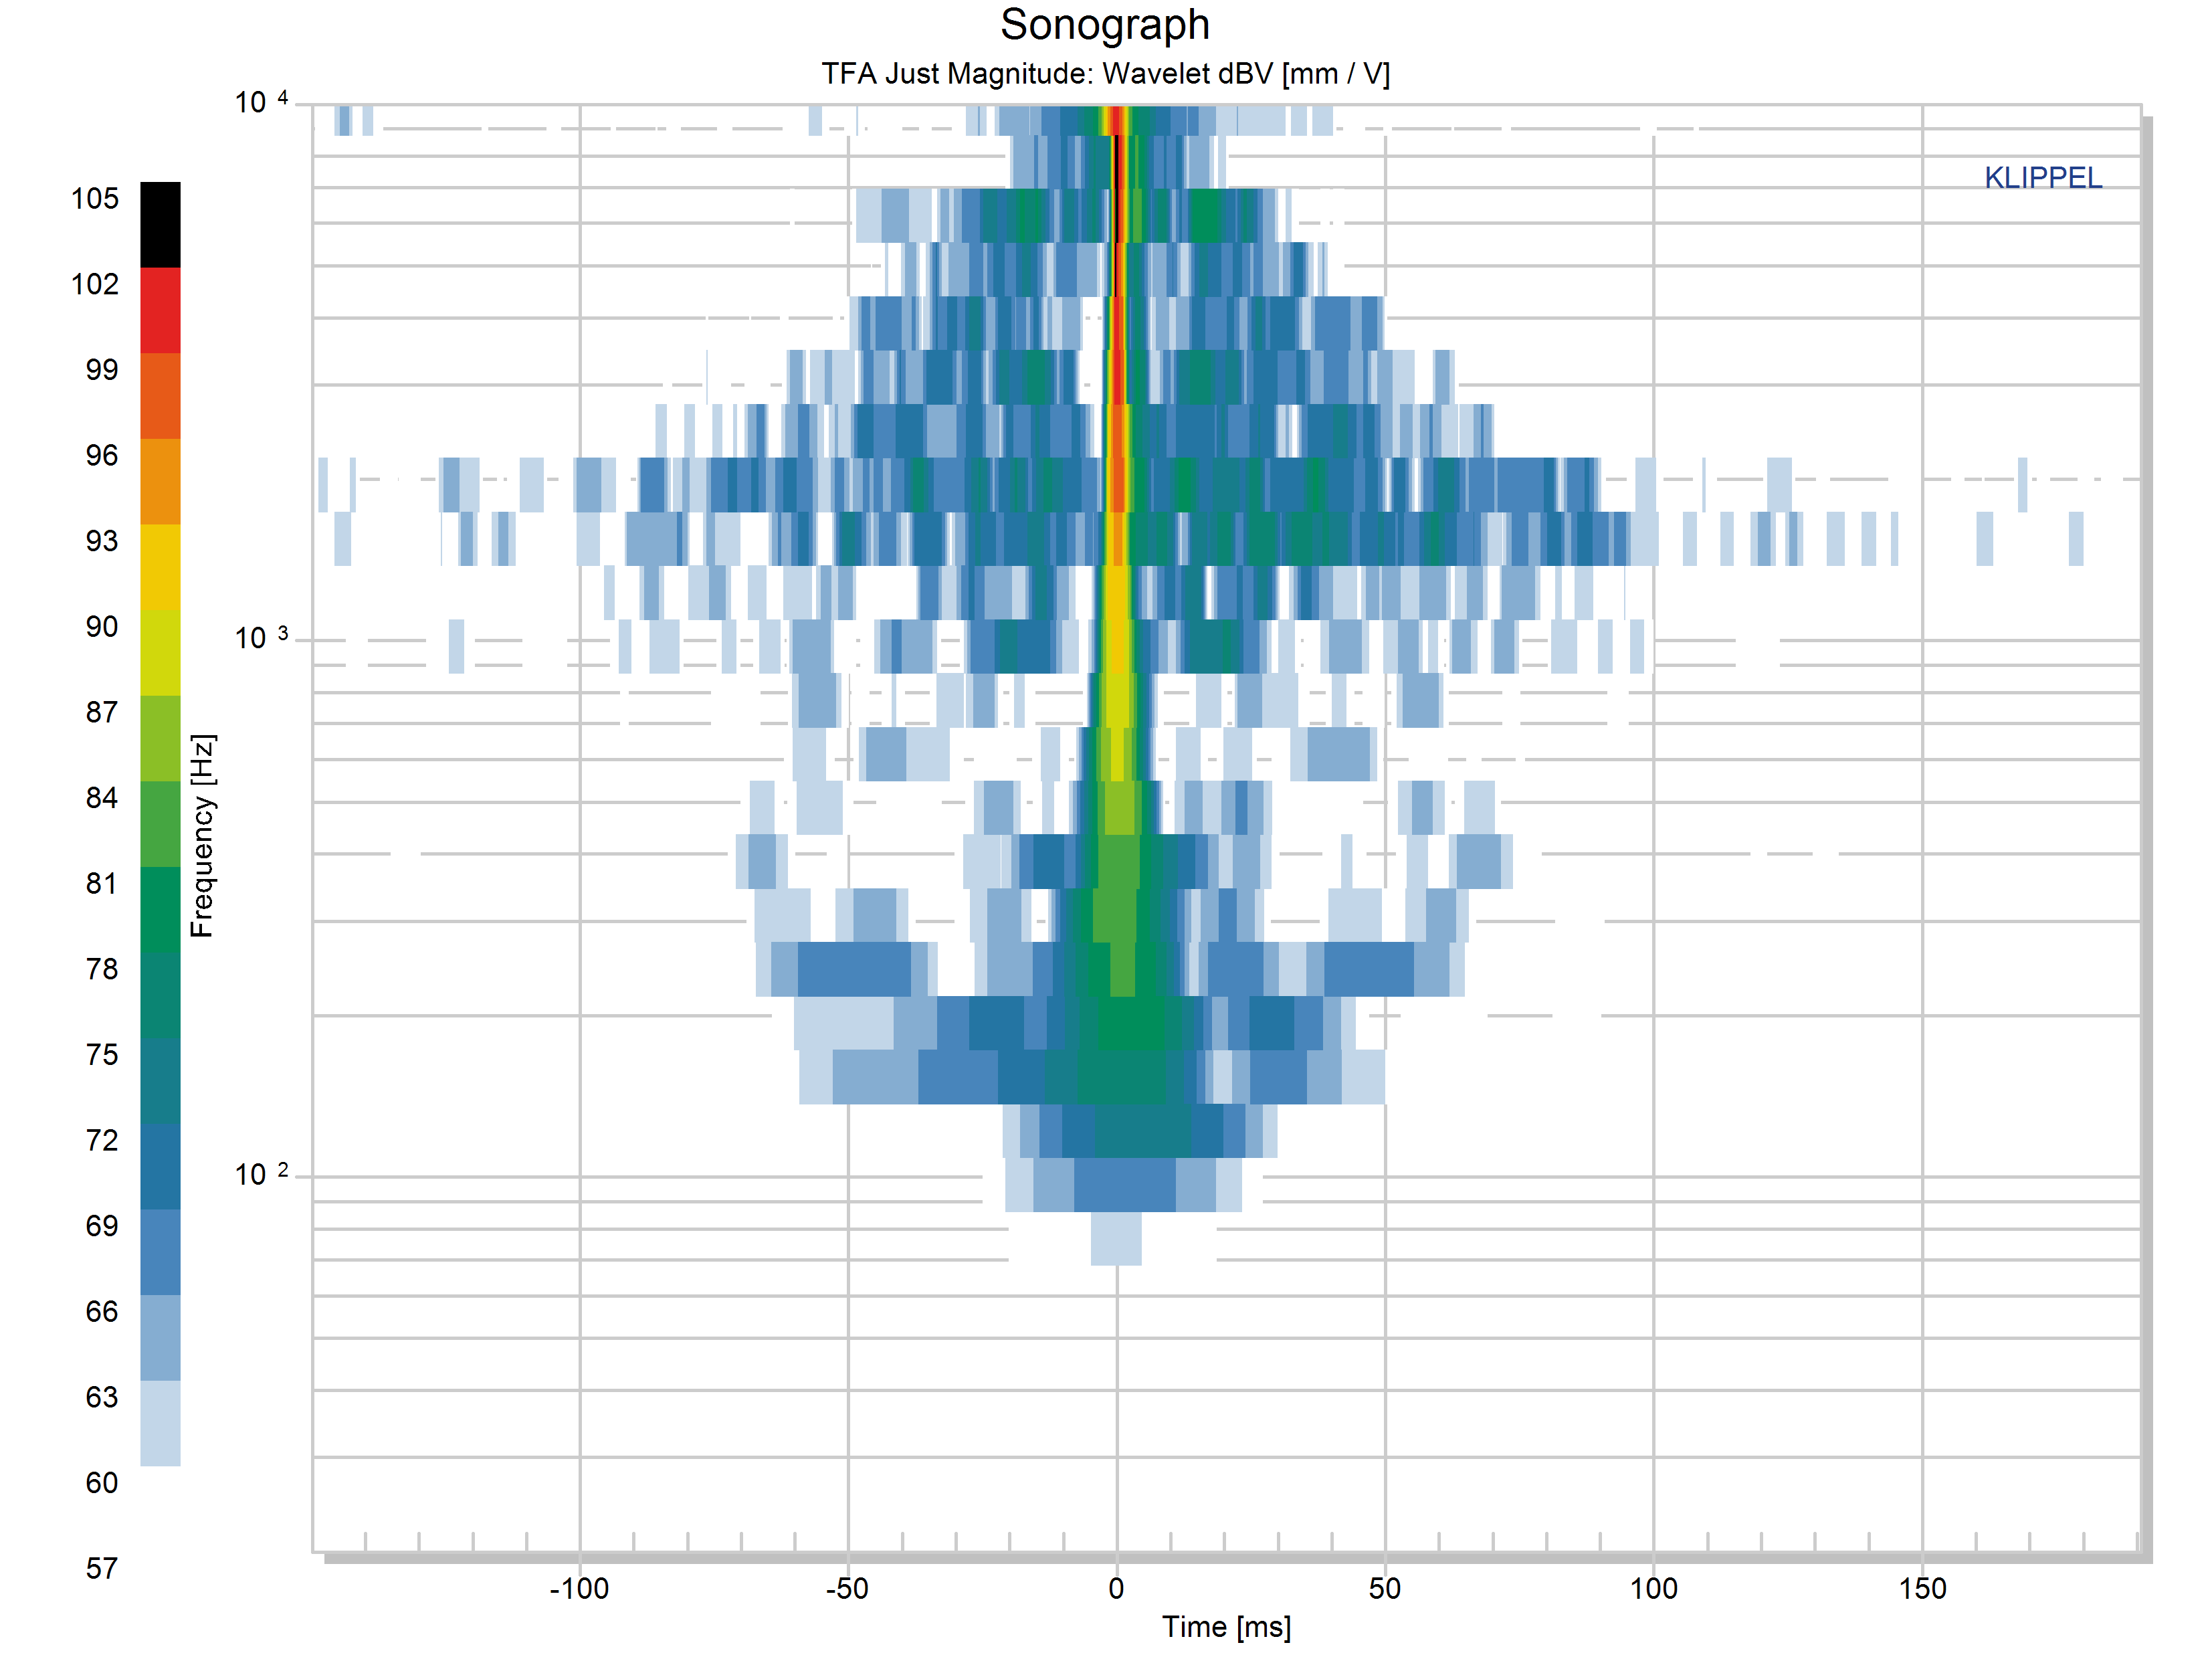
\includegraphics[width=\textwidth]{RoomComp/Sonograph_MagFilt} 
    \captionsetup{hypcap=false} 
	\captionof{figure}{Filter on magnitude} 
	\label{fig:comp_mag}
\end{center}
\end{minipage}
\begin{minipage}{0.33333333\textwidth}
\begin{center}
	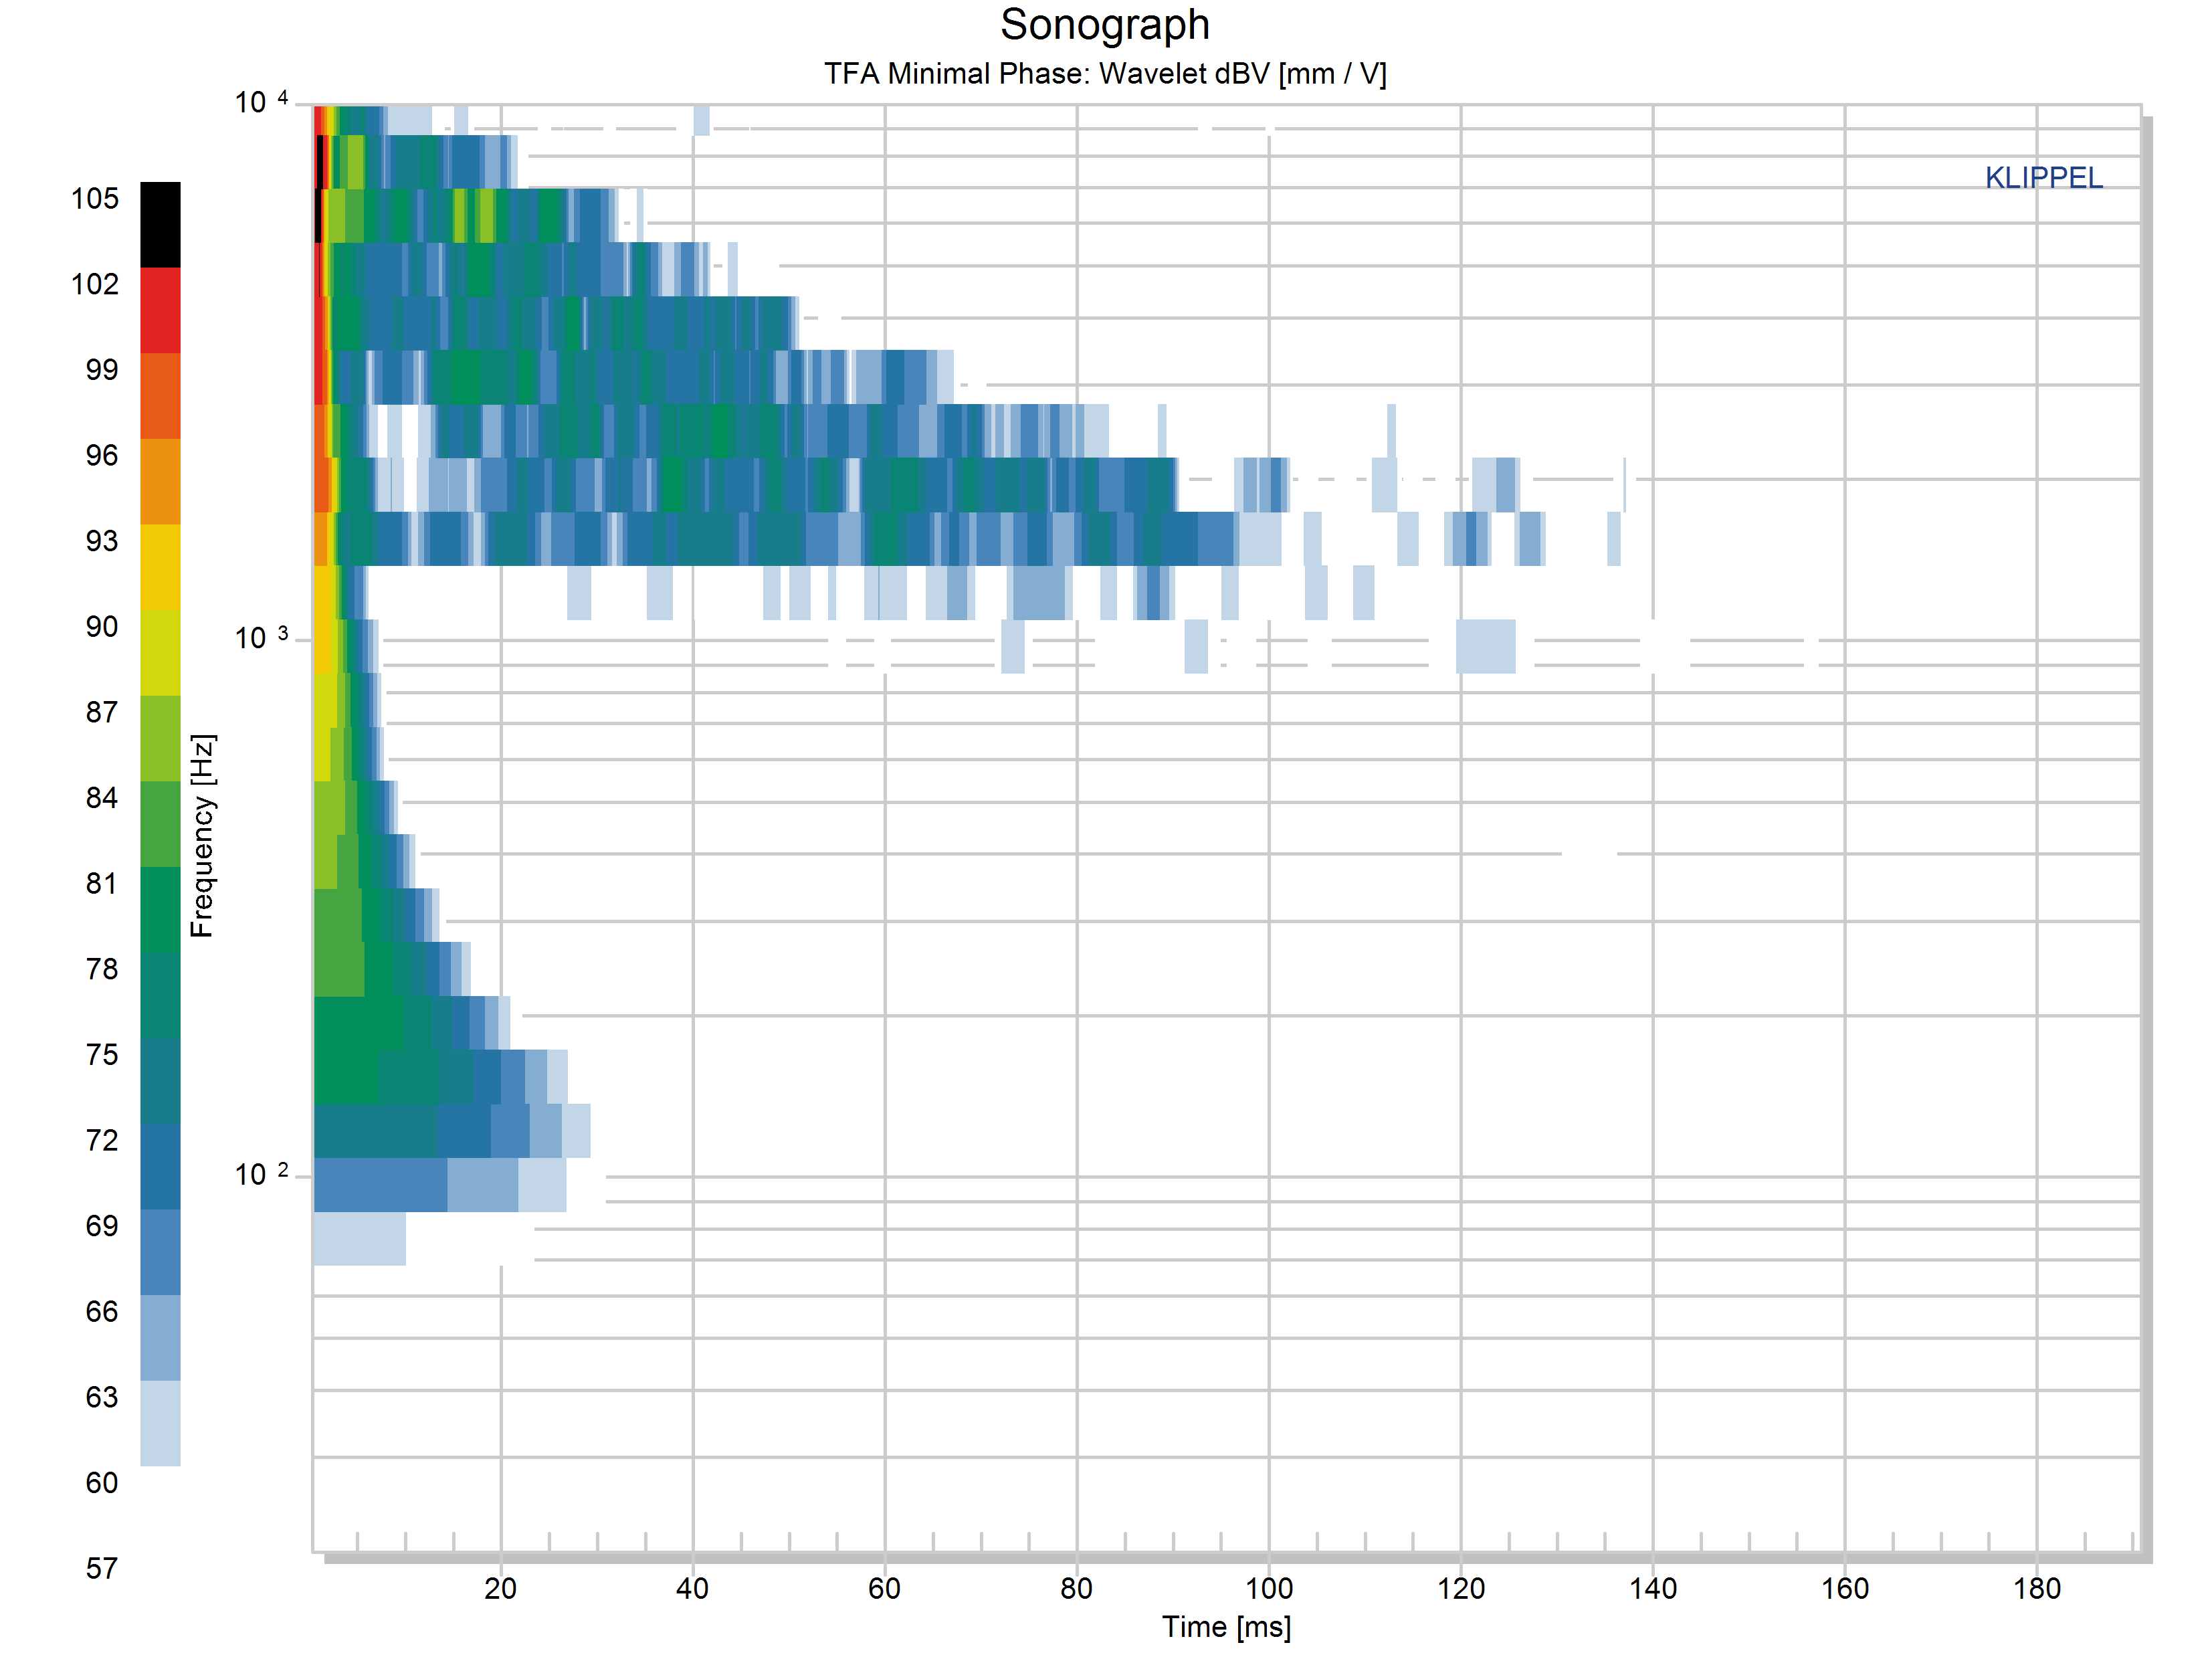
\includegraphics[width=\textwidth]{RoomComp/Sonograph_MinPhase} 
    \captionsetup{hypcap=false} 
	\captionof{figure}{Filter with minimal phase} 
	\label{fig:comp_minphase}
\end{center}
\end{minipage}
\begin{minipage}{0.33333333\textwidth}
\begin{center}
	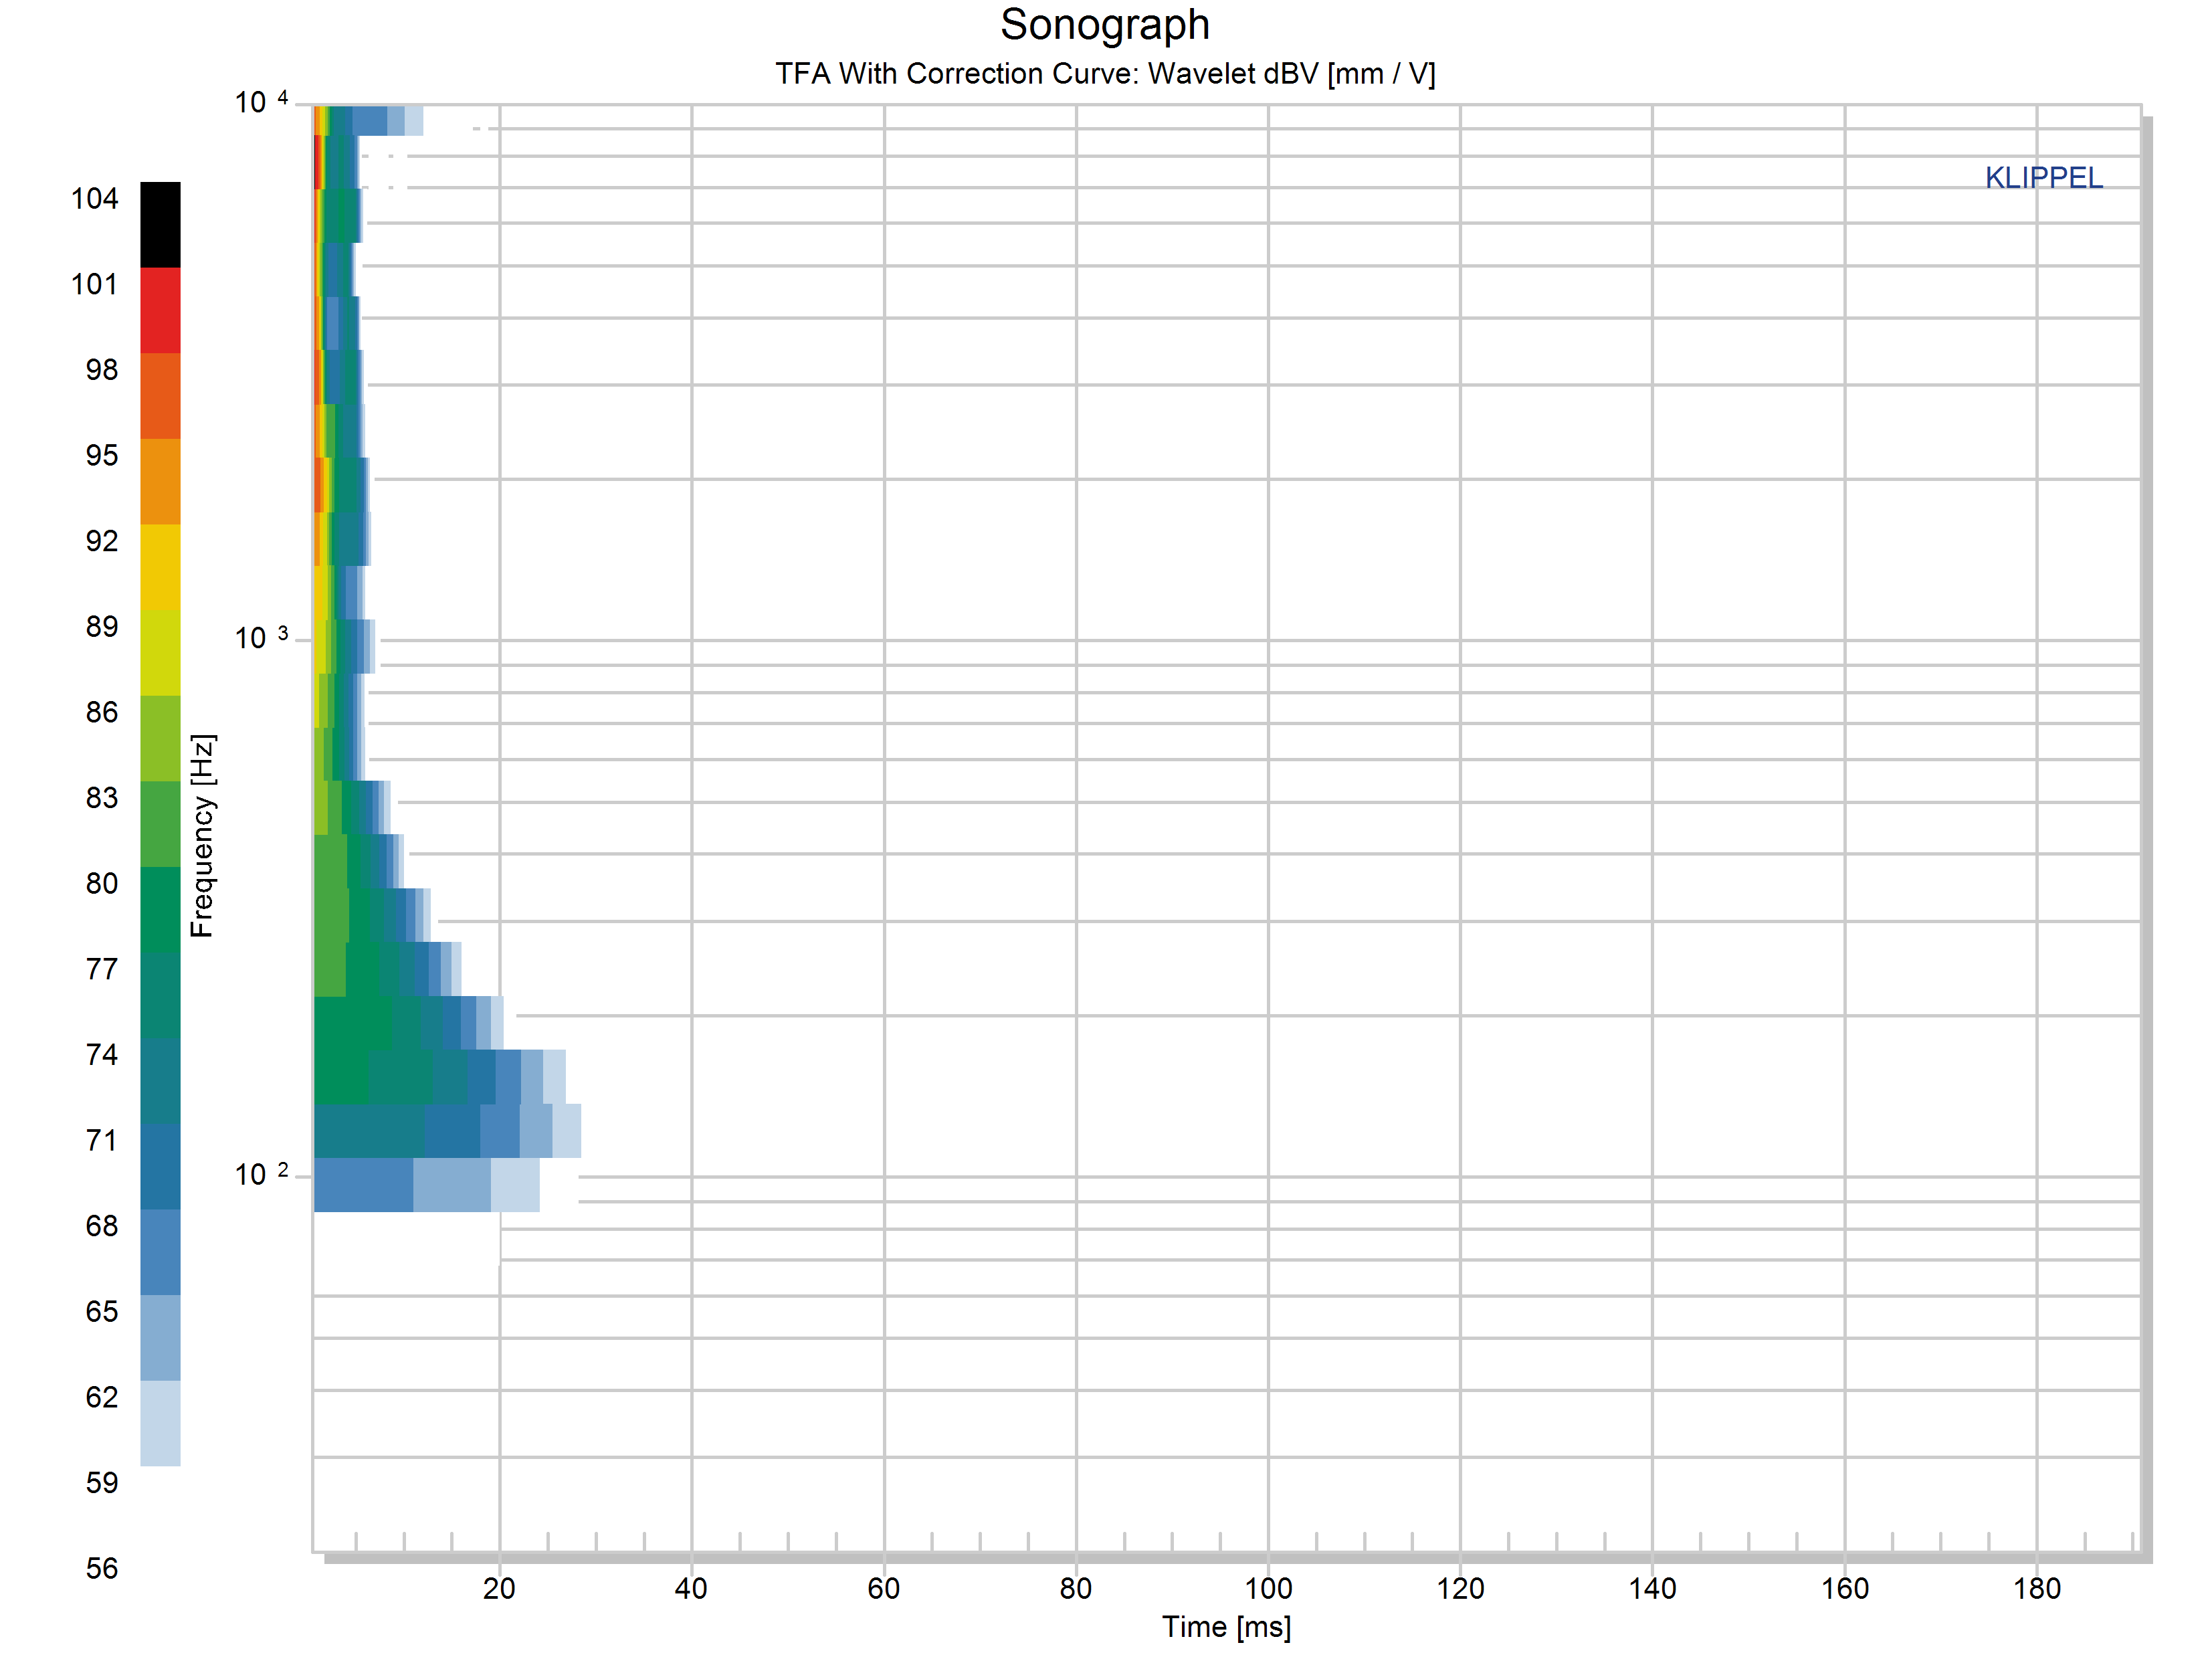
\includegraphics[width=\textwidth]{RoomComp/Sonograph_RoomCor} 
    \captionsetup{hypcap=false} 
	\captionof{figure}{Filter with LFR} 
	\label{fig:comp_RoomCor}
\end{center}
\end{minipage}
\vspace{0.1cm}

Figure \ref{fig:comp_RoomCor} presents the Time-Frequency Analysis (TFA) of three different methods to perform a room correction, applied on a measurement of a speaker's transfer function: the left graph shows a TFA when a pre-filter have been applied on the magnitude of the Transfer Function, the middle graph is when the pre-filter contains the minimal phase that have been reconstructed from the cepstrum of the Transfer Function, and the right graph shows the TFA of the transfer function filtered by the Room Correction curve calculated using the Low-Frequency Reference method described in \citep[][sect.~4]{aeswb}.\\

The pre-filtering on the magnitude of the transfer function does not take in account other informations of the measurements, and filters the phase out, generating strange artifacts visible on the TFA. \\
When using a pre-filter with a reconstructed minimal phase, the accuracy of the correction is enhanced in low frequency. However, this methods is still polluted by noise in high frequencies. \\
The calculated room correction method provides the best result: by using a reference curve provided by a measurement of the speaker using the NFS, the phase response of the room can be removed completely, removing completely the artifacts visible on the TFA. 

\section{Measurements}

In order to have compare different curve and have different references, several measurement campaigns have been held. The first measurements have been done using the NFS, with speakers mounted on the baffle. The speakers have then been measured in a tetrahedral text box \citep[see][]{tetbox}. Then, some measurements have been done in the anechoic room of the Technical University in Dresden. Finally, some measurement of the speakers in free air and in a QC test box provided by Klippel have been conducted. 

\subsection{10 cm woofer}

The first measured device is a 10 cm woofer (see \ref{spkrlib:10cm}). 

\subsection{16 cm fullband driver}

\subsection{Influence of the load}

Measuring in a closed box will influence the behavior of the speaker by modifying the load of air the membrane have to compress. This effect have already been observed in low frequency for both speakers (see \textbf{REFERENCE TO CURVES}). The aim is now to evaluate how critically this load influences the speaker, and how to correct this effect.\\

To estimate this, a Large Signal Identification (LSI) have been performed on both speakers to estimate the non-linear parameters in the box, and in free air. The parameter of interest is the stiffness of the speaker's membrane $K_{ms}$. \\

\begin{minipage}{0.5\textwidth}
\begin{center}
	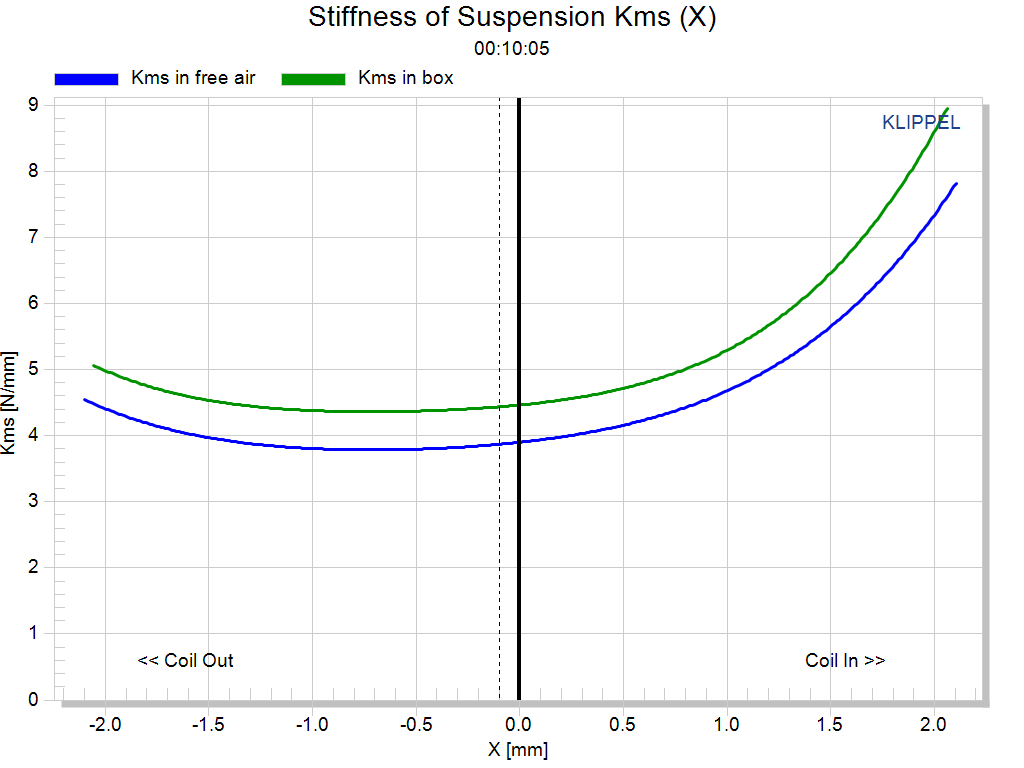
\includegraphics[width=0.7\textwidth]{RoomComp/Kms_10cm} 
    \captionsetup{hypcap=false} 
	\captionof{figure}{$K_{ms}$ of 10cm woofer} 
	\label{fig:kms10}
\end{center}
\end{minipage}
\begin{minipage}{0.5\textwidth}
\begin{center}
	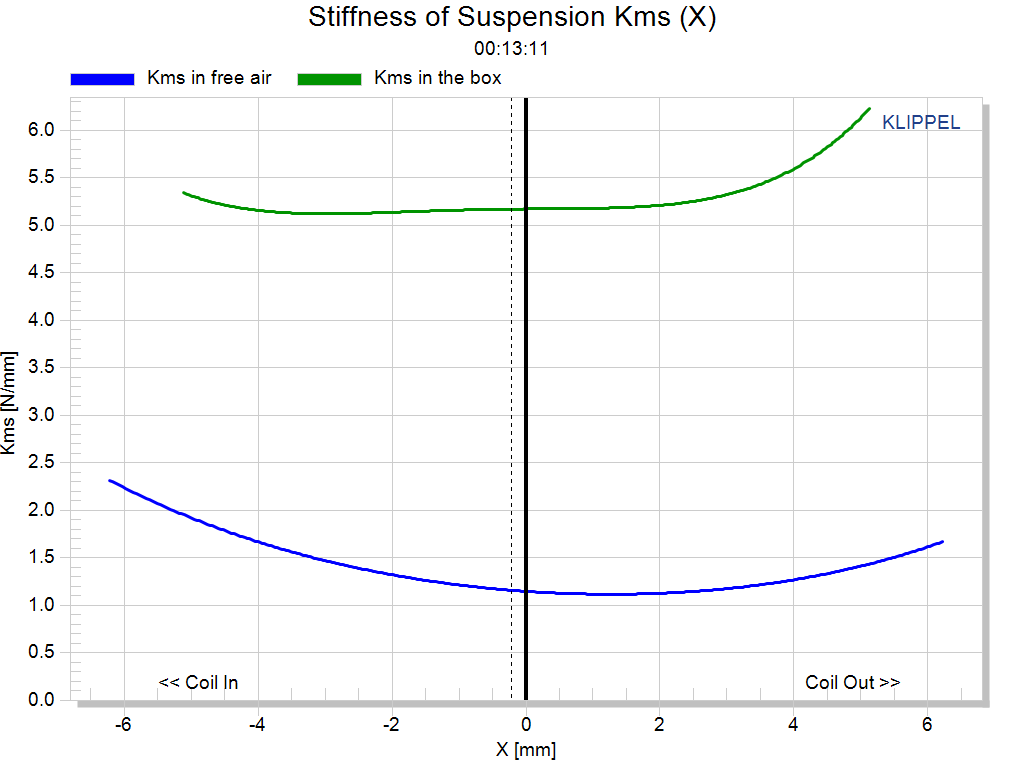
\includegraphics[width=0.7\textwidth]{RoomComp/Kms_12cm} 
    \captionsetup{hypcap=false} 
	\captionof{figure}{$K_{ms}$ of 16cm fullband} 
	\label{fig:kms12}
\end{center}
\end{minipage}
\vspace{0.1cm}

Figure \ref{fig:kms10} presents the measurements of $K_{ms}$ of the 10cm woofer (see appendix \ref{spkrlib:10cm}). The curve has the same shape for both measurements, but the $K_{ms}$ is higher for the measurement in the box: since the speaker has to compress more air to generate the same Sound Pressure Level. The difference between the two curves is 0.5 N/mm. \\

Figure \ref{fig:kms12}  presents the measurements of $K_{ms}$ of the 16cm fullband driver (see appendix \ref{spkrlib:12cm}). The curves changes its shape drastically, and the offset between the configurations is almost 3 N/mm. This difference could be explained by the size of the speaker, which might be too big for the test box model used: the volume of the box being too small for this driver, the compression effect is exaggerated, generating high variations of the stiffness $K_{ms}$. 

\subsection{Influence of microphone position}

Investigating the influence of the microphone position allows to deduce how critical this parameter is, and how to ensure a correct microphone positioning. Several measurements of the 10cm woofer (see appendix \ref{spkrlib:10cm}) have been performed for different microphones positions. A schematic of the positions is given in appendix \ref{Curves:InfluMicPos}. 

\begin{center}
	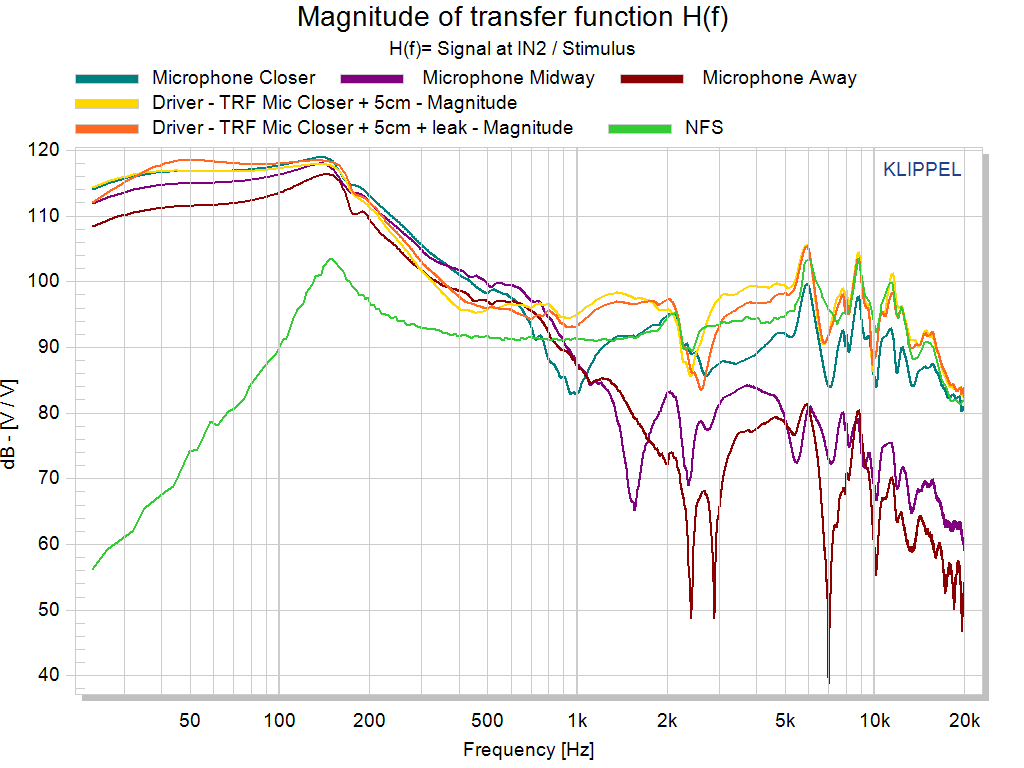
\includegraphics[width=0.55\textwidth]{RoomComp/MicPos_TRF_Compa} 
    \captionsetup{hypcap=false} 
	\captionof{figure}{Comparison of transfer function for different microphone positions} 
	\label{fig:micposcomp}
\end{center}

Figure \ref{fig:micposcomp} presents the results for different microphone positions, compared with the results from the NFS (light green curve). The closer the microphone is to the membrane, and the more agreement there is between the NFS and the box measurement. 


\section{Room Correction solutions}

In order to correct the previous measurements and ensure a good measurement in the tetrahedral test box, several solution of Room Correction methods have been investigated. The aim is to generate a single Room Correction function, valid for all speaker, up to the cut-off frequency of the box.

\subsection{D. B. Keele method for Far Field extrapolation}

D. B. Keele presented a simplified method for extrapolation of the Far Field pressure of a device by measuring in the near field. The theory is given in the article \textit{Low-Frequency Loudspeaker Assessment by Nearfield Sound-Pressure Measurement} \citep[see][]{dkeele}. The Near - Far pressure relation is given in equation \ref{eq:nfpressure}.

\begin{equation}
p_{N} = \frac{2r}{a} \cdot p_{F}
\label{eq:nfpressure}
\end{equation}
\myequations{Near-Far field pressure relation}

Where $p_{N}$ and $p_{F}$ are respectively the Near and Far field pressures, $r$ is the distance between the center of the driver's membrane and the measuring point, and $a$ the radius of the driver's membrane.\\

The results of this extrapolation, after implementation in SciLab, are given in appendix \ref{Curves:dbkFF}. 

\section{Discussion}



%--------------------------------------------------------------
%	CONCLUSION
%--------------------------------------------------------------
% \chapter*{Conclusion}
% \addcontentsline{toc}{chapter}{Conclusion}

% Several investigations have been done in the context of this report and gave significant results. \\~\\

% On a more personal note, working at Klippel GmbH have been a very enjoyable experience that gives me more insight about the real functioning of a company and what to expect from my future. I am thrilled to have had the opportunity to conduct this work, and very satisfied with the variety of the tasks I was assigned to, which included programming, measuring, and research to draw conclusion from my experiments. \\

% Thank you for reading my work.

%--------------------------------------------------------------
%	BIBLIOGRAPHY
%--------------------------------------------------------------

\bibliography{bibli}
\bibliographystyle{abbrv}

\nocite{*}

%--------------------------------------------------------------
%	APPENDIX
%--------------------------------------------------------------

\begin{appendices}

		% GANTT CHART
\chapter{Organization of the work}
\pagenumbering{roman}

The following will present the work schedule I have followed, what work have been done and when it have been started and finished. This is presented in the following GANTT chart.

\begin{center}
	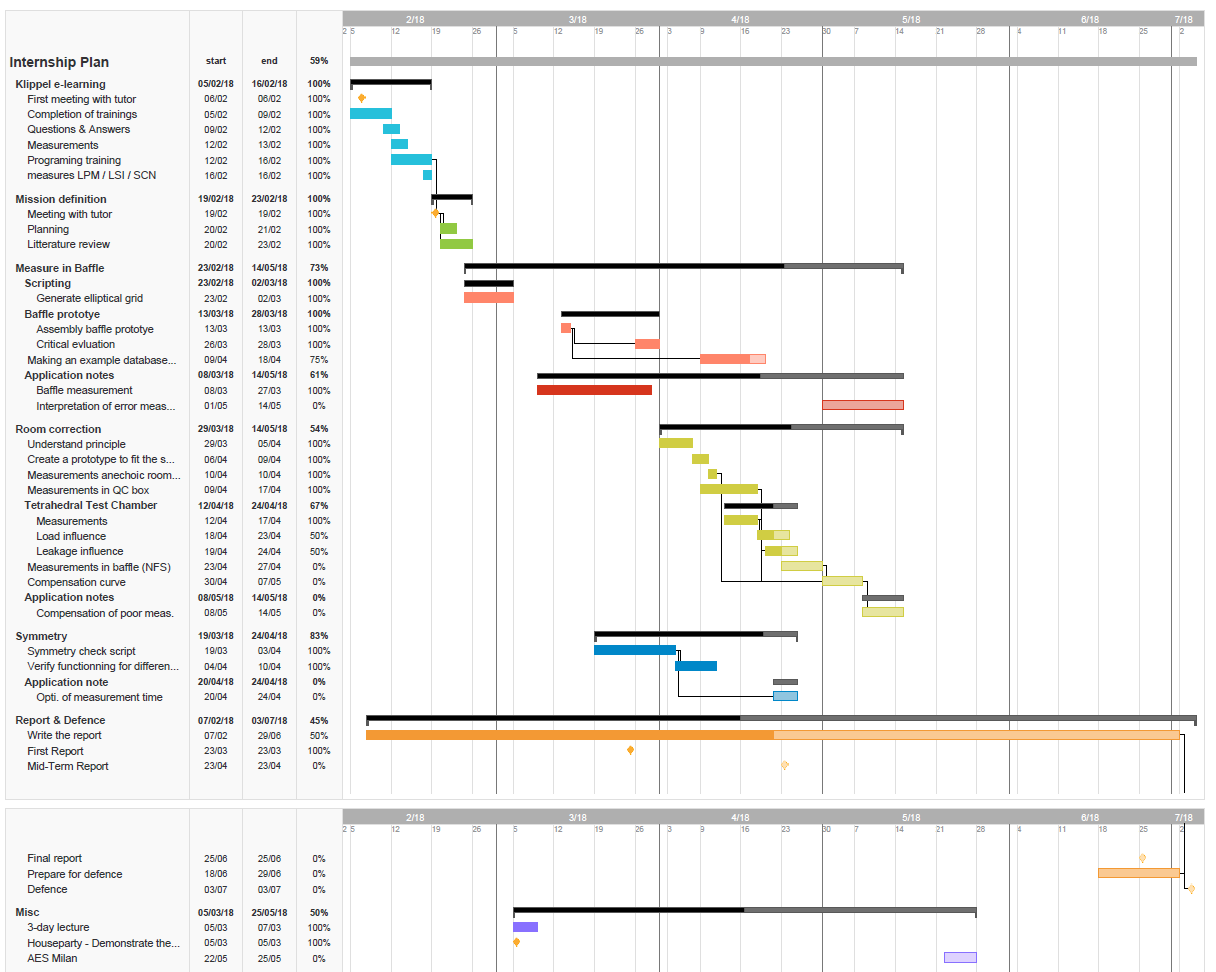
\includegraphics[width=\textwidth]{Appendix/Plan1} 
\end{center}

		% Symmetry
\chapter{Equations for symmetry condition on complex coefficients of spherical wave expansion}
\label{chap:sym}

\textit{\textbf{NOTE}: the presented equations are coming from the reference \cite{aeshs}. They are displayed in this report for a more comfortable reading experience and for reference, and I do not take any credits for the presented results.} \\

\begin{minipage}{0.5\textwidth}
\begin{center}
	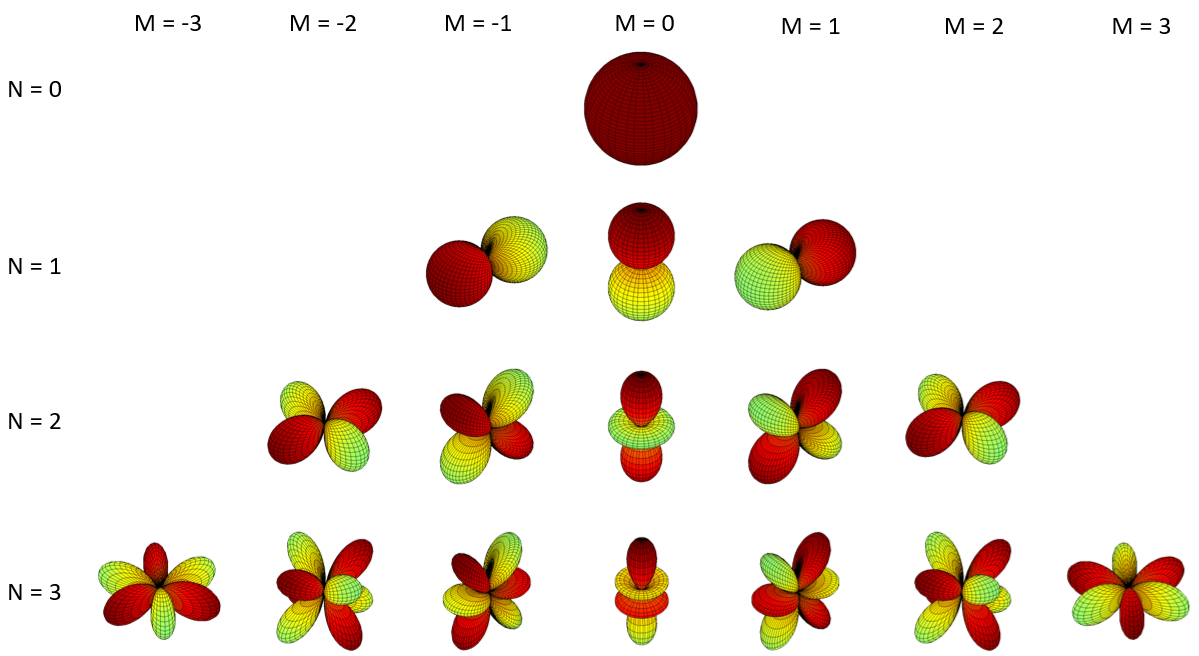
\includegraphics[scale=0.25]{Appendix/Spherical_Harmo}
    \captionsetup{hypcap=false}
    \captionof{figure}{Spherical Harmonics}
    \label{fig:Sph_Harmo}
\end{center}
\end{minipage}
\begin{minipage}{0.5\textwidth}
\vspace{0.2cm}
The solution of the three-dimensional wave equation in spherical coordinates can be described by a spherical wave expansion given by equation \ref{eq:sphwvexp}.The free-field transfer function of a loudspeaker can be expressed by only considering the direct sound (outgoing wave) in equation \ref{eq:sphwvexp} and is expressed in equation \ref{eq:ffHf}.\\

Figure \ref{fig:Sph_Harmo} presents a visual representation of the first few spherical harmonics, and their orders (n,m) (\textit{all images presented in this chapter are courtesy of W. Klippel, from the presentation \cite{lect2018}}). \\~\\~\\~\\
\end{minipage}


\textbf{Influence of symmetry on coefficients} \\

\begin{minipage}{0.7\textwidth}
Rotational symmetry (see figure \ref{fig:rotsym}) is observed for many circular drivers and is the simplest type of symmetry as a lot of coefficients are vanishing according to the relation given by equation \ref{eq:Crotsym}.

\begin{equation}
C_{mn} = 0 \; \; \; \;  m \neq 0
\label{eq:Crotsym}
\end{equation}
All m $\neq$ 0 coefficients are vanishing, meaning that only m = 0, n = n+1 coefficients have to be estimated. \\

Once the coefficients have been estimated, s symmetry factor S can be estimated. For rotation symmetry, $S_{rs}$ is given by equation \ref{eq:Srs}.

\begin{equation}
S_{rs} = 1-\frac{\sum_{n=1}^{N}\sum_{s=1}^{n}\left | C_{sn} \right |^{2}}{\sum_{n=0}^{N}\sum_{m=-n}^{n} C_{mn}^{2}}
\label{eq:Srs}
\end{equation}
\myequations{Symmetry factor for rotational symmetry}

\end{minipage}
\begin{minipage}{0.3\textwidth}
\begin{center}
	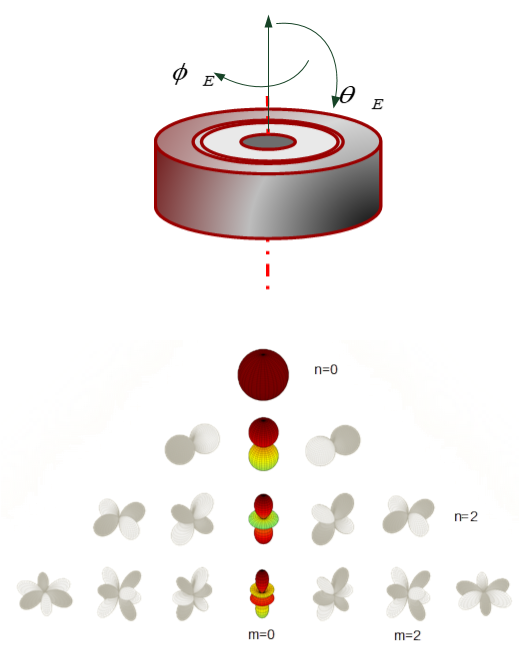
\includegraphics[width=\textwidth]{Appendix/Rot_Sym}
    \captionsetup{hypcap=false}
    \captionof{figure}{Rotational symmetry}
    \label{fig:rotsym}
\end{center}
\end{minipage}

\vspace{1cm}

\begin{minipage}{0.7\textwidth}
Dual plane symmetry (see figure \ref{fig:dualpsym}) is mostly observed in 2-way closed box systems, and make half of the coefficients vanish according to the relation given by equation \ref{eq:Cdpsym}. 

\begin{equation}
C_{mn}(f) = C_{-mn}(f)R_{m}(f) \; \; \; \;  m = 2s; \; s =1, 2, 3...
\label{eq:Cdpsym}
\end{equation}

Where Rm represents a complex symmetry parameter, expressed in equation \ref{eq:Rm}.

\begin{equation}
R_{m}(f) = (-1)^{m+1}(\textup{sin}(m \phi _{s}(f)) + i\textup{cos}(m \phi _{s}(f)))^{2}
\label{eq:Rm}
\end{equation}
\myequations{Complex symmetry parameter}
With $\phi _{s}$ is the symmetry axis; and $m$ the suborder of the coefficient under study.
\end{minipage}
\begin{minipage}{0.3\textwidth}
\begin{center}
	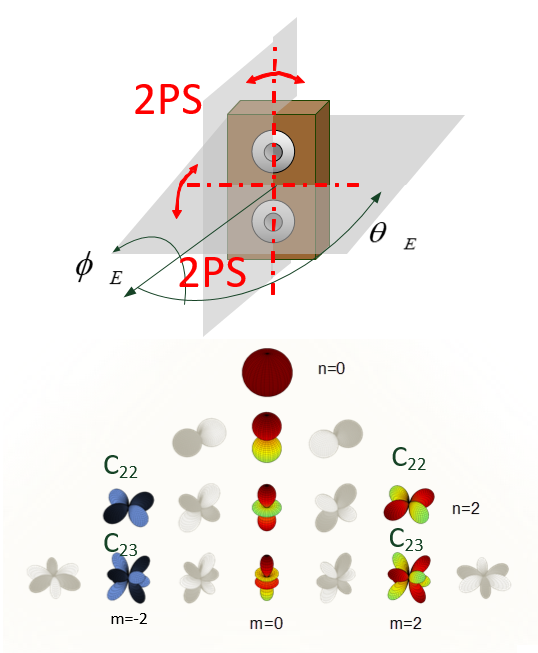
\includegraphics[width=\textwidth]{Appendix/Dual_Plane_Sym}
    \captionsetup{hypcap=false}
    \captionof{figure}{Dual Plane symmetry}
    \label{fig:dualpsym}
\end{center}
\end{minipage}\\


If the symmetry axes ($\Phi _{e}, \Theta _{e}$ are aligned with the coordinate system, equation \ref{eq:Cdpsym} can be simplified to the relation given in equation \ref{eq:Cdpsymb}.

\begin{equation}
C_{mn}(f) = C_{-mn}(f) \; \; \; \;  m = 2s; \; s =1, 2, 3...
\label{eq:Cdpsymb}
\end{equation}

The symmetry factor for the Dual Plane symmetry is then given by equation \ref{eq:Sdps}.


\begin{equation}
S_{dps} = 1-\frac{\sum_{n=1}^{N}\sum_{s=1}^{n/2}\left | (-1)^{2s}C_{(2s)n} - C_{(2s)n}\right |^{2} + \sum_{n=1}^{N}\sum_{s=0}^{n/2}\left | C_{(2s+1)n}\right |^{2}}{\sum_{n=0}^{N}\sum_{m=-n}^{n} C_{mn}^{2}}
\label{eq:Sdps}
\end{equation}
\myequations{Symmetry factor for dual-plane symmetry}

\vspace{1cm}

\begin{minipage}{0.7\textwidth}
Baffle symmetry is when the Device Under Test is mounted on a baffle (see figure \ref{fig:bafflesym}), and make half of the coefficient vanish according to the relation given by equation \ref{eq:Cbsym}.

\begin{equation}
C_{mn} = 0 \; \; \; \; \; \; n-m \, \neq \, 2s \: \: s \in \mathbb{Z}
\label{eq:Cbsym}
\end{equation}

The symmetry factor is then given by equation \ref{eq:Sbs}.

\begin{equation}
S_{bs} = 1-\frac{\sum_{n=1}^{N}\sum_{s=0}^{n/2}\left | C_{(2s)n} \right |^{2}}{\sum_{n=0}^{N}\sum_{m=-n}^{n} C_{mn}^{2}}
\label{eq:Sbs}
\end{equation}
\myequations{Symmetry factor for baffle symmetry}
\end{minipage}
\begin{minipage}{0.3\textwidth}
\begin{center}
	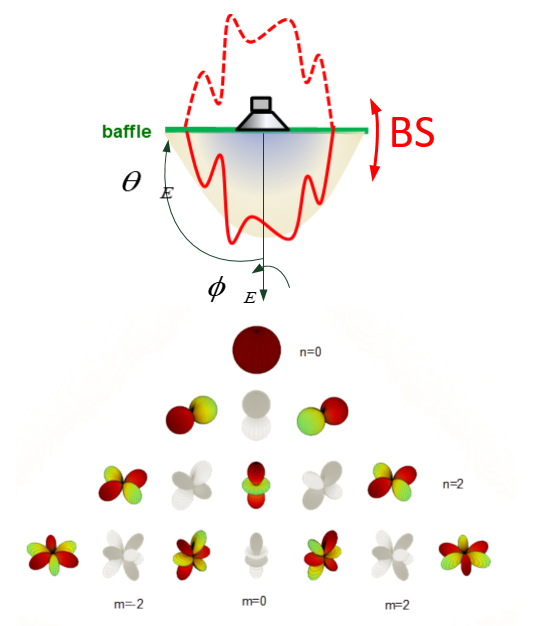
\includegraphics[width=\textwidth]{Appendix/Baffle_Sym}
    \captionsetup{hypcap=false}
    \captionof{figure}{Baffle symmetry}
    \label{fig:bafflesym}
\end{center}
\end{minipage}

\vspace{1cm}

\begin{minipage}{0.7\textwidth}
Single plane symmetry is the most common in loudspeakers systems using 2 or more drivers. This symmetry can be between the left and right side of the DUT, as presented in figure \ref{fig:singplsym}; but also between the top and bottom of the DUT. Only the coefficients on the left side have to be estimated. The coefficients of the right side are linked to the left side by the relation given by equation \ref{eq:spsym}.

\begin{equation}
C_{mn} = C_{-mn}(f)R_{m}(f) \; \; \; \textup{with} \; \; 0\leq m; \; \; \; 0\leq n\leq N
\label{eq:spsym}
\end{equation}

It should be noted that depending of the type of symmetry (left/right or top/bottom), $R_{m}$ will change, modifying the relation between the coefficients. \\

The symmetry factor is then given by equation \ref{eq:Ssps}.

\begin{equation}
S_{sps} = 1-\frac{\sum_{n=1}^{N}\sum_{m=1}^{n}\left | (-1)^{m}(f) C_{-mn}-C_{mn} \right |^{2}}{\sum_{n=0}^{N}\sum_{m=-n}^{n} C_{mn}^{2}}
\label{eq:Ssps}
\end{equation}
\myequations{Symmetry factor for single-plane symmetry}
\end{minipage}
\begin{minipage}{0.3\textwidth}
\begin{center}
	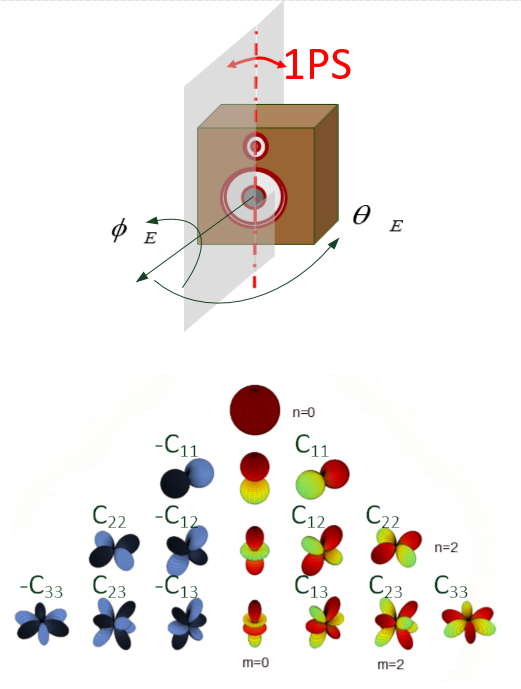
\includegraphics[width=\textwidth]{Appendix/Single_Plane_Sym}
    \captionsetup{hypcap=false}
    \captionof{figure}{Single Plane symmetry}
    \label{fig:singplsym}
\end{center}
\end{minipage}

\newpage

\textbf{Implementation} \\

The following code shows hoy these equations have been implemented in SciLab.\\
\textit{\textbf{NOTE}: This program have been simplified by removing some functions, the aim being to demonstrate how the algorithm calculating the coefficients based on symmetry conditions works.}

\lstset{language=SCilab} 
\begin{lstlisting}
//------------------------------------------------MAIN FUNCTION
function OnRun()
// Loading the datas
Cout = load('Cout.txt');
Cin  = load('Cin.txt');
f    = load('f.txt');

N = sqrt(size(Cout,1))-1; // Number of points

// Constants 
P0  = 10^(-12);		      //reference sound power
rho = 1.204;		         //density of the air
c   = 343;		            //speed of sound
k   = 2*%pi*f'/c;	         //wavenumber k
A   = 4*%pi*radius^2; 

// Rotational symmetry (example)
[Csym_ROT, Crest_DPS, powOut_rot, powRestOut_rot] = CheckSymAll(Cout, N, f, 'ROT');
ROT_TotOut_FF  = [f' 10*log10(powOut_rot' ./(rho*c*k^2)/P0)];        // Total outgoing power 
ROT_OutRest_FF = [f' 10*log10(powRestOut_rot' ./(rho*c*k^2)/P0)];    // Rest of outgoing power
ROT_SymFactor_FF = [f' (abs(powOut_rot./(powOut_rot+powRestOut_rot)))'];    // Symmetry factor
endfunction // OnRun

//--------------------------------------------Find the coeffs for different symmetries
function [Csym, Crest, power_sym, power_rest] = CheckSymAll(C, N, f, SymType)
   // CheckSymAll: calculates the coeff according the different symmetry conditions
   // Inputs:     C: coefficients to find symmetry on 
   //             N: number of iterations 
   //             f: frequency vector
   //             SymType: a string with the symmetry types. 
   //	          Allowed values are: 'ROT', 'DPS', 'BS', 'SPS_LR', 'SPS_TB' 
   //                      representing respectively Rotational Symmetry, Dual Plane Symmetry, 
   //                      Baffle Symmetry, Single Plane Symmetry (Top/Bottom), Single 
   //                      Plane Symmetry (Left/Right)
   // Outputs:    Csym: coefficients of the symmetry condition
   //             Crest: rest of coefficients = all coeffs - Csym
   //             power_sym: power of the symmetry coefficients
   //             power_rest: power of the rest coeffcients   
   
   // Initialization of matrices (all coeffs, left and right coefficients)
   Csym = zeros(size(C,'r'),size(C,'c'));
   Csym_l = zeros(size(C,'r'),size(C,'c'));  
   Csym_r = zeros(size(C,'r'),size(C,'c'));
   
   // Calculation of coefficient according to symmetry condition assumed
   select SymType
   
   case 'ROT' 	// Rotational symmetry
      [nm] = calc_nm_index(N*ones(f), 1);                      
      [n, m] = order_suborder(nm(:,1));   // Finding the equivalent nm value 
      
      // Finding the equivalent index value for m=0
      for i = 1:size(m,'r')
         index(i) = GetIndex(n(i), m(i));
         if m(i)==0 then
            Csym(index(i),:) = C(index(i),:);   // If m=0 we put the value in C in the Csym
         end
      end
      
   case 'DPS'	// Dual Plane symmetry
      [nm] = calc_nm_index(N*ones(f), 5);                
      [n, m] = order_suborder(nm(:,1));   // Finding the equivalent n and m values
      
      index_row = GetIndex(n, m);
      Csym_l(index_row,:) = C(index_row,:);  // Filling the Coeffs of the left with the correct data
      
      // Finding the equivalent m value and index for the right side
      // Calculation of corresponding coefficient
      for i = 1:size(m,'r')
         m_r(i) = -1*m(i);
         index_r(i) = GetIndex(n(i), m_r(i));
         index_l(i) = GetIndex(n(i), m(i));
         
         if isequal(index_l(i),index_r(i))==%F then
            Csym_r(index_r(i),:) = (1)*C(index_l(i),:);
         end
      end
      Csym = Csym_l + Csym_r; 
      
   case 'BS'	// Baffle symmetry
      [nm] = calc_nm_index(N*ones(f), 2);    // For baffle
      [n, m] = order_suborder(nm(:,1));   
      
      index_row = GetIndex(n, m);                 
      Csym(index_row,:) = C(index_row,:); 
      
   case 'SPS_LR'	// Single Plane (L/R) symmetry
      [nm] = calc_nm_index(N*ones(f), 4);                // For single plane symmetry
      [n, m] = order_suborder(nm(:,1));   
      
      index_row = GetIndex(n, m);
      Csym_l(index_row,:) = C(index_row,:); 
      
      for i = 1:size(m,'r')
         m_r(i) = -1*m(i);
         index_r(i) = GetIndex(n(i), m_r(i));
         index_l(i) = GetIndex(n(i), m(i));
         
         if isequal(index_l(i),index_r(i))==%F then
            Csym_r(index_r(i),:) = C(index_l(i),:)*(-1)^(m(i));
         end
      end
      Csym = Csym_l + Csym_r;
      
   case 'SPS_TB'	// Single Plane (T/B) symmetry
      [nm] = calc_nm_index(N*ones(f), 4);                // For single plane symmetry
      theta_sym = %pi/2; // symmetry angle  
      [n, m] = order_suborder(nm(:,1));  
      
      index_row = GetIndex(n, m);
      Csym_l(index_row,:) = C(index_row,:); 
      
      for i = 1:size(m,'r')
         m_r(i) = -1*m(i);
         index_r(i) = GetIndex(n(i), m_r(i));
         index_l(i) = GetIndex(n(i), m(i));
         
         Rm(i) = ((-1)^(m_r(i)+1))*(sin(m_r(i)*theta_sym) + %i*cos(m_r(i)*theta_sym))^2;
         if isequal(index_l(i),index_r(i))==%F then
            Csym_r(index_r(i),:) = C(index_l(i),:)*Rm(i);
         end
      end
      Csym = Csym_l + Csym_r;
   end
   
   // Calculation of the rest 
   Crest = C - Csym;
   
   // Calculation of power
   power_sym  = sum(abs(Csym).^2,1);    // Estimating the power of sym
   power_rest = sum(abs(Crest).^2,1);   // Estimating the power of rest
endfunction
\end{lstlisting}

		% Speaker library
\chapter{Speaker library}
\label{chap:spk_lib}

\section{10 cm woofer}
\label{spkrlib:10cm}

\begin{minipage}{0.6\textwidth}
This speaker is a 10 cm (4'') woofer from Phillips, designed for PSS usage (car speaker). A picture is shown in figure \ref{fig:spkr_lib_10cm}\\ 
The Thiele \& Small  parameters of this speaker have been measured using the Klippel scanning system and are presented in table \ref{tab:TnS_10cmWoofer}. 
\end{minipage}
\begin{minipage}{0.4\textwidth}
\begin{center}
	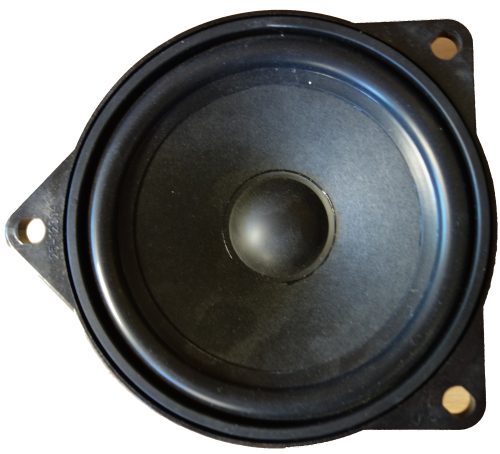
\includegraphics[scale=1]{Appendix/Round_Spkr}
    \captionsetup{hypcap=false}
    \captionof{figure}{10 cm woofer}
    \label{fig:spkr_lib_10cm}
\end{center}
\end{minipage}




\begin{table}[ht]
\centering
\begin{tabular}{|c|c|c|c|c|c|c|c|c|c|}
\hline
\begin{tabular}[c]{@{}c@{}}Re \\{[}$\Omega${]}\end{tabular} & \begin{tabular}[c]{@{}c@{}}Fs\\{[}Hz{]}\end{tabular} & \begin{tabular}[c]{@{}c@{}}Mms\\  {[}g{]}\end{tabular} & \begin{tabular}[c]{@{}c@{}}Cms\\{[}mm/N{]}\end{tabular} & \begin{tabular}[c]{@{}c@{}}Rms\\  {[}kg/s{]}\end{tabular} & Bl    & Qms   & Qes   & Qts   & \begin{tabular}[c]{@{}c@{}}Vas\\  {[}L{]}\end{tabular} \\ \hline
3.28                                                                        & 145.8                                                                 & 5.492                                                                 & 0.217                                                                    & 1.619                                                                    & 3.197 & 3.108 & 1.614 & 1.063 & 1.89                                                                  \\ \hline
\end{tabular}
\caption{T \& S parameters of 10cm woofer}
\label{tab:TnS_10cmWoofer}
\end{table}

\section{Oval speaker}
\label{spkrlib:oval}

\begin{minipage}{0.6\textwidth}
This speaker is a 23 cm x 15 cm fullband speaker. A picture is shown in figure \ref{fig:spkr_lib_Oval}.\\
The T\&S parameters of the speaker were not given and haven't been measured.

\end{minipage}
\begin{minipage}{0.4\textwidth}
\begin{center}
	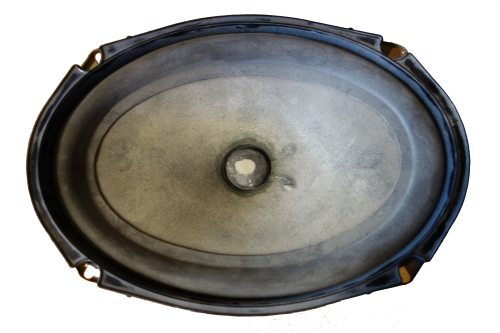
\includegraphics[scale=1]{Appendix/Oval_Spkr}
    \captionsetup{hypcap=false}
    \captionof{figure}{Oval speaker}
    \label{fig:spkr_lib_Oval}
\end{center}
\end{minipage}

\section{16 cm fullband speaker}
\label{spkrlib:12cm}

This speaker is a 16 cm fullband speaker. The T\&S parameters are given in table \ref{tab:TnS_FullBand}.

\begin{table}[ht]
\centering
\begin{tabular}{|c|c|c|c|c|c|c|c|c|c|}
\hline
\begin{tabular}[c]{@{}c@{}}Re \\ {[}$\Omega${]}\end{tabular} & \begin{tabular}[c]{@{}c@{}}Fs\\{[}Hz{]}\end{tabular} & \begin{tabular}[c]{@{}c@{}}Mms\\  {[}g{]}\end{tabular} & \begin{tabular}[c]{@{}c@{}}Cms\\ {[}mm/N{]}\end{tabular} & \begin{tabular}[c]{@{}c@{}}Rms\\  {[}kg/s{]}\end{tabular} & Bl    & Qms   & Qes   & Qts   & \begin{tabular}[c]{@{}c@{}}Vas\\  {[}L{]}\end{tabular} \\ \hline
5.39                                                                        & 52                                                                    & 14.630                                                                & 0.641                                                                    & 0.724                                                                    & 8.112 & 6.599 & 0.391 & 0.369 & 11.6093                                                               \\ \hline
\end{tabular}
\caption{T\&S parameters of 12cm fullband driver}
\label{tab:TnS_FullBand}
\end{table}

\section{2-way diagonal speaker}
\label{spkrlib:BnO}

\begin{minipage}{0.6\textwidth}
This 2-way speaker presents the particularity of having its tweeter and woofer mounted diagonally (see figure \ref{fig:2wayDiagSpkr}). The measurements have been focused on the tweeter of this speaker, and the reference axis for the measure have been setted along the "measurement axis" showed on figure \ref{fig:2wayDiagSpkr}.\\

The manufacturer didn't gave many information about the speakers, and the only thing known about these tweeters is that they are 3/4''.

\end{minipage}
\begin{minipage}{0.4\textwidth}
\begin{center}
	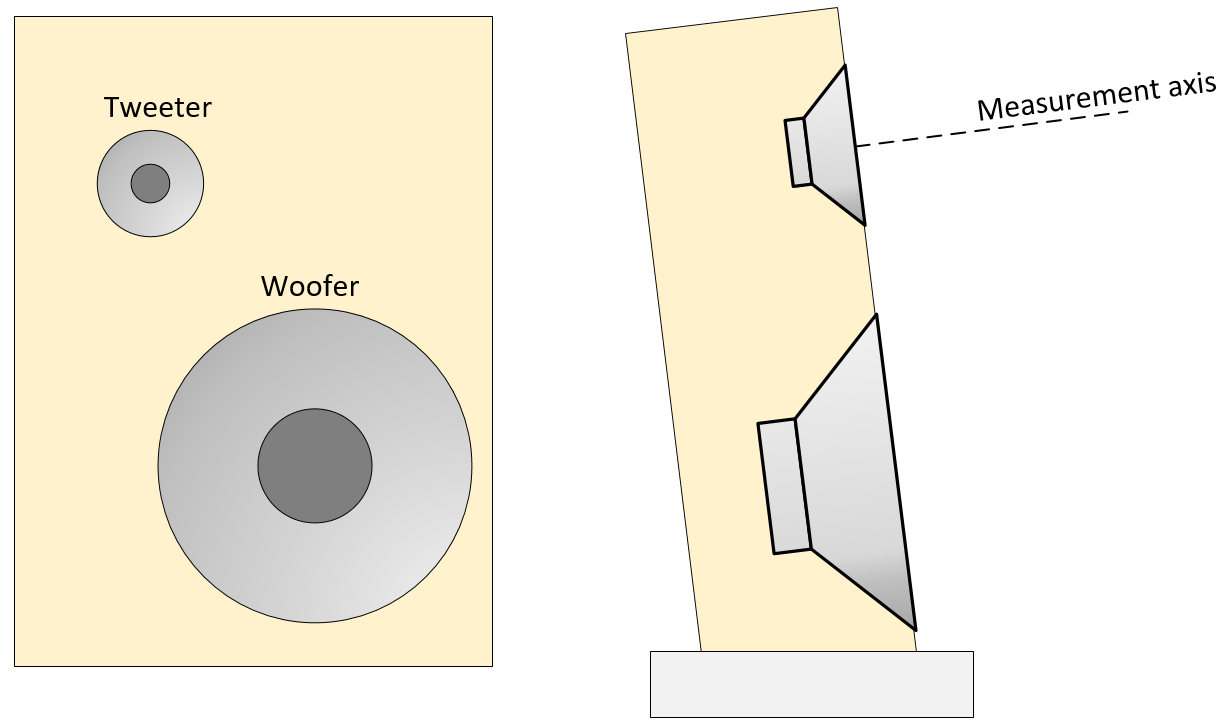
\includegraphics[scale=0.2]{Sym/Spkr_BmO}
    \captionsetup{hypcap=false}
    \captionof{figure}{2-way diagonal speaker}
    \label{fig:2wayDiagSpkr}
\end{center}
\end{minipage}

\section{18'' woofer}

\begin{minipage}{0.6\textwidth}
This speaker is an 18'' JBL WPU1805-X woofer. The T\&S parameters were provided by the manufacturer and are presented in table \ref{tab:TnS_BigBooy}. 
\begin{center}
\begin{tabular}{|c|c|c|c|c|c|}
	\hline
	\begin{tabular}[c]{@{}c@{}}Re \\ {[}$\Omega${]}\end{tabular} & \begin{tabular}[c]{@{}c@{}}Fs\\  {[}Hz{]}\end{tabular} & 	Qms   & Qes  & Qts & \begin{tabular}[c]{@{}c@{}}Vas\\  {[}L{]}\end{tabular} \\ \hline
	5.6                                                          & 35                                                     & 	21.09 & 0.73 &  0.70   & 293                                                    \\ \hline
\end{tabular}
\captionsetup{type=table} \caption{T\&S parameters of 18'' woofer}
\label{tab:TnS_BigBooy}
\end{center}
\end{minipage}
\begin{minipage}{0.4\textwidth}
\begin{center}
	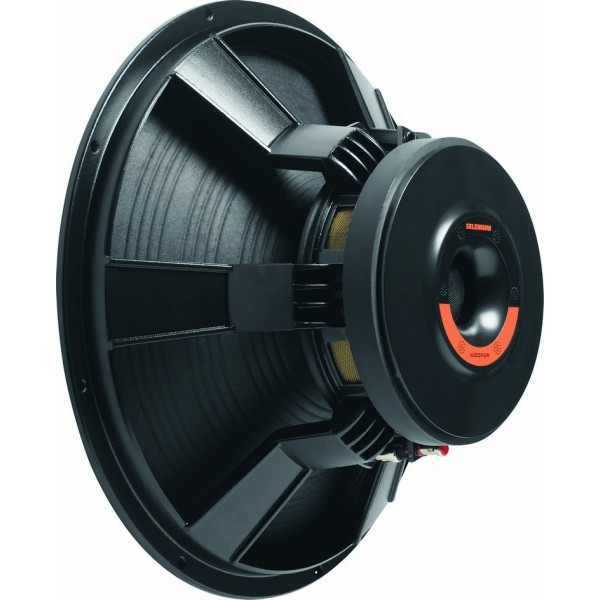
\includegraphics[width=0.6\textwidth]{Appendix/bigwoof}
    \captionsetup{hypcap=false}
    \captionof{figure}{18'' woofer}
    \label{fig:bigwoof}
\end{center}
\end{minipage}




		% Additional curves
\chapter{Additional figures}
This appendix aims to present additional figures that could not be presented in the corpus of this report because of their size, or lacked of relevancy for the discussions. To simplify the navigation, the titles of the section will be the same as the tittle of the chapters this figures are complemented with. 


\section{Baffle measurement}
\subsection{Estimation of baffle influence}
\label{Curves:BaffleInfluence}

\begin{center}
	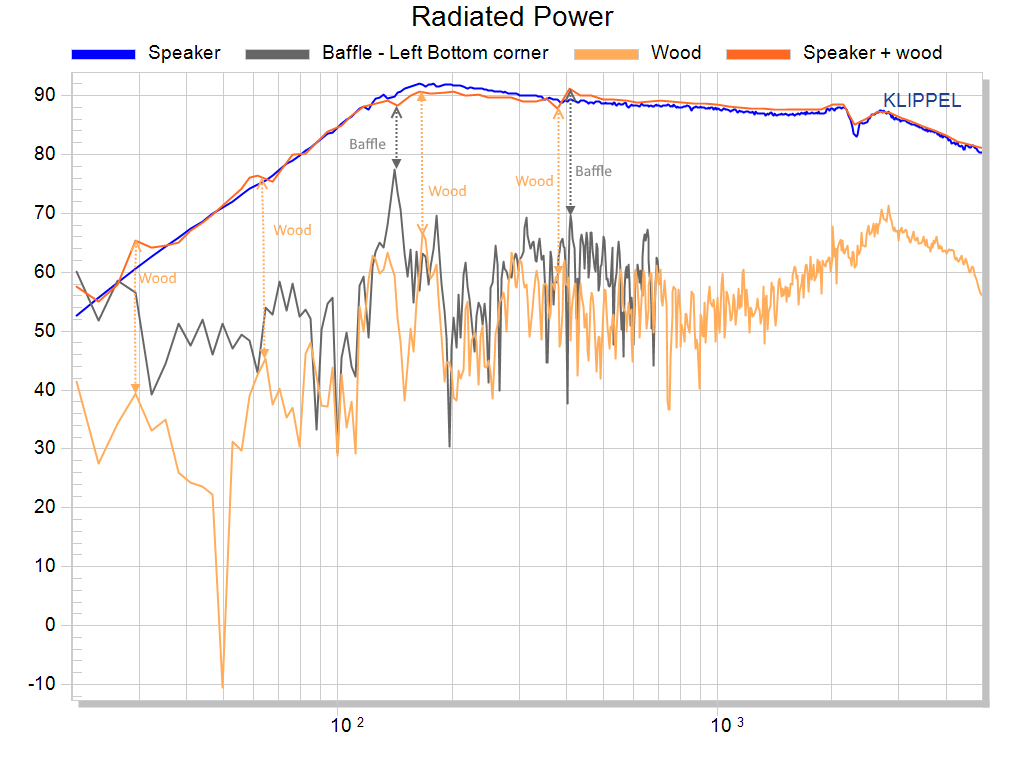
\includegraphics[width=0.9\textwidth]{Appendix/Vib_RadPow}
    \captionsetup{hypcap=false}
    \captionof{figure}{Radiated Powers at 1m for different measurement points on the baffle}
    \label{Curves:Baffle_RadPow}
\end{center}

\begin{center}
	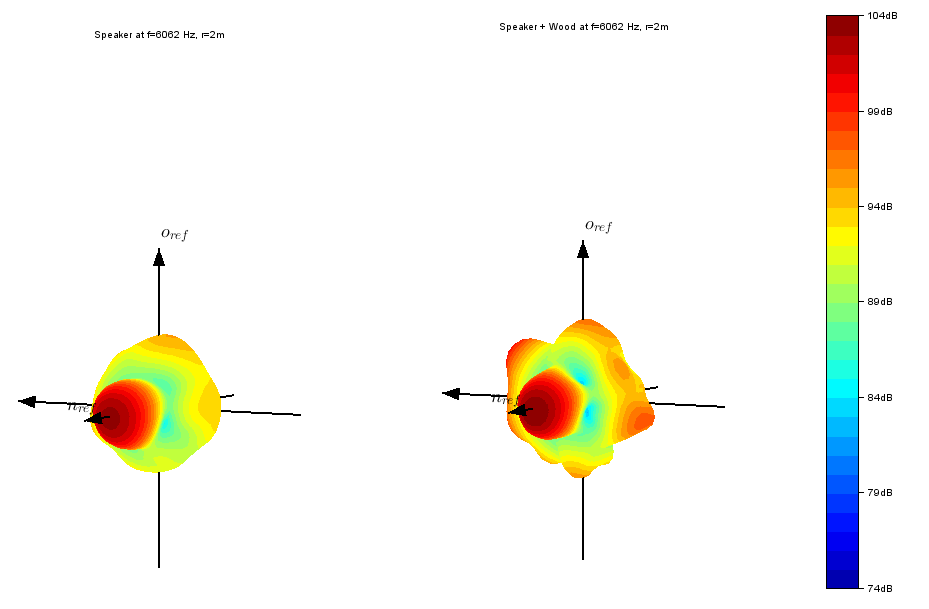
\includegraphics[width=0.8\textwidth]{Appendix/compa_baffle_Vib_Balloon}
    \captionsetup{hypcap=false}
    \captionof{figure}{Comparison of directivity balloon for the speaker and speaker + wood contribution}
    \label{Curves:Baffle_BalloonComp}
\end{center}

\begin{center}
	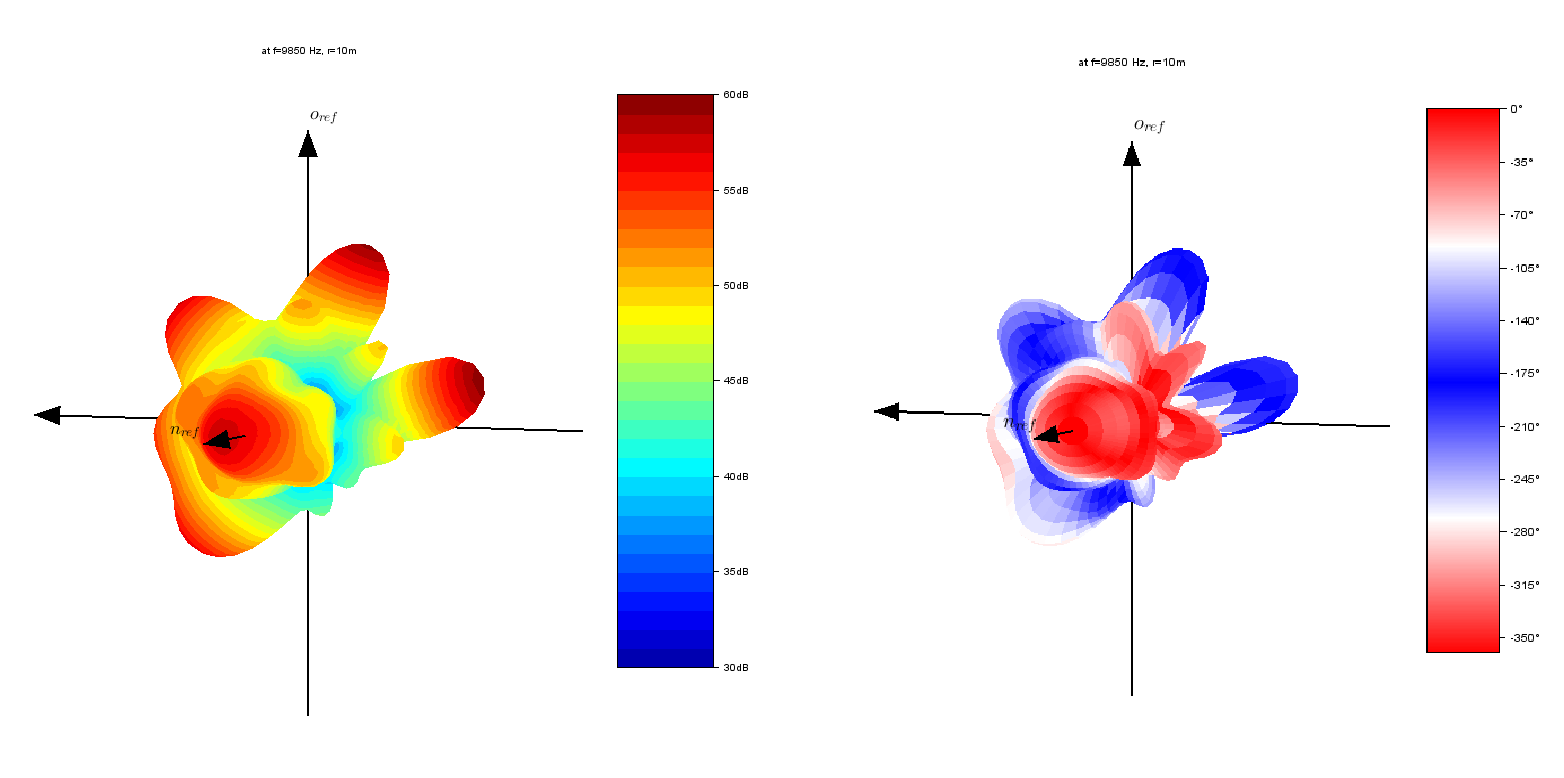
\includegraphics[width=0.8\textwidth]{Appendix/compa_baffle_Vib_SpkrWood_All}
    \captionsetup{hypcap=false}
    \captionof{figure}{Directivity balloon and phase balloon at 9.58 kHz of the speaker + wood}
    \label{Curves:Baffle_BalloonWood}
\end{center}



\section{Measurement time optimization}
\subsection{Oval speaker}
\label{Curves:oval}
\begin{center}
	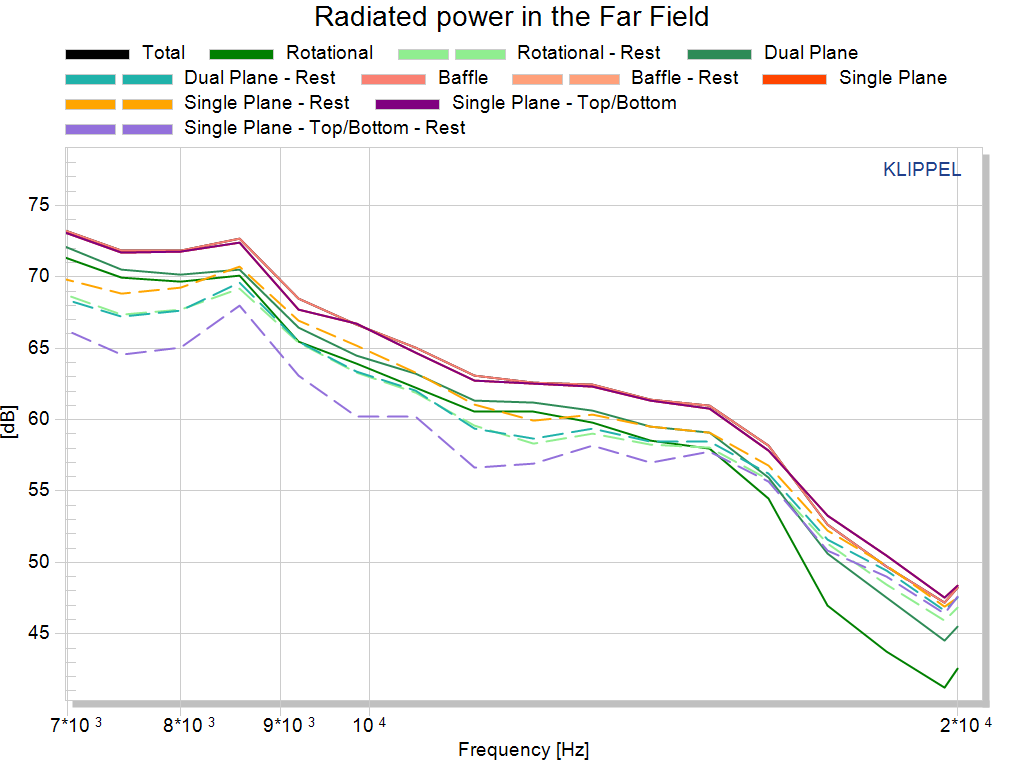
\includegraphics[width=0.9\textwidth]{Appendix/Rad_Pow_OvalSpkr_ZoomHF}
    \captionsetup{hypcap=false}
    \captionof{figure}{Radiated Powers for oval speaker: zoom on 7 - 20 kHz}
\end{center}

\subsection{2-way "diagonal" speaker}

\begin{center}
	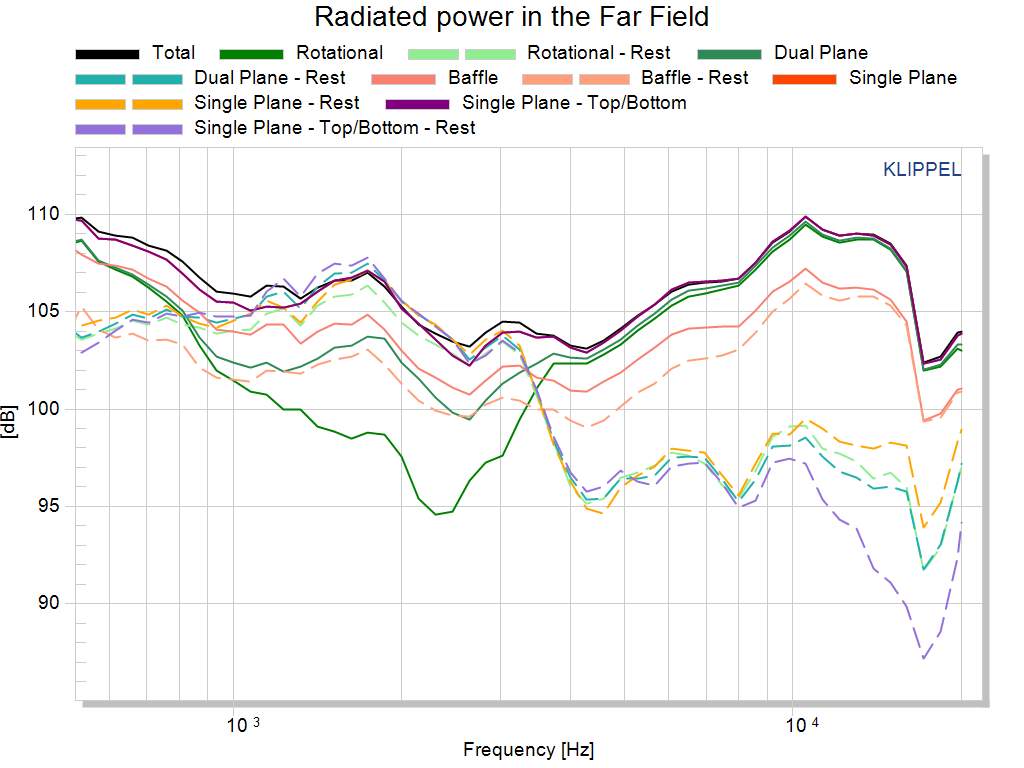
\includegraphics[width=0.9\textwidth]{Appendix/Rad_Pow_BnO_ZoomHF}
    \captionsetup{hypcap=false}
    \captionof{figure}{Radiated Powers for 2-way diagonal speaker: zoom on crossover frequency}
    \label{Curves:2way}
\end{center}


\section{Room Correction}

\subsection{Measurements}
\subsubsection{Influence of microphone position}
\label{Curves:InfluMicPos}
\begin{center}
	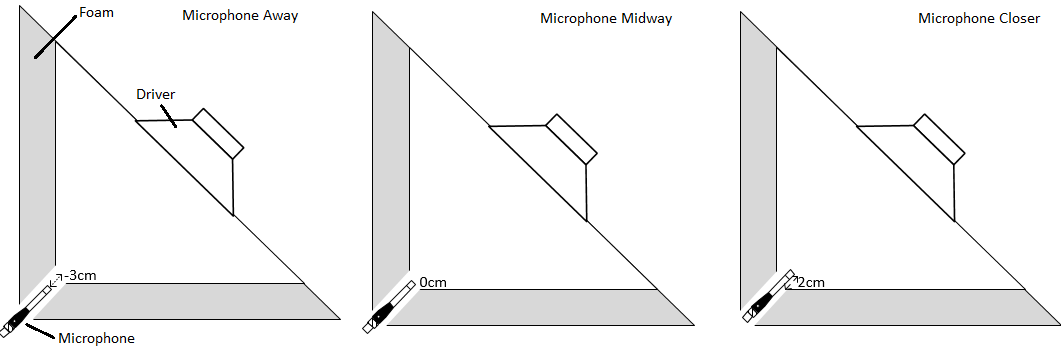
\includegraphics[width=\textwidth]{Appendix/micpos} 
    \captionsetup{hypcap=false} 
	\captionof{figure}{Different microphones positions} 
	\label{fig:micpos_schema}
\end{center}

\subsection{Room Correction solutions}

\subsubsection{D. B. Keele method for Far Field extrapolation}
\label{Curves:dbkFF}

\begin{center}
	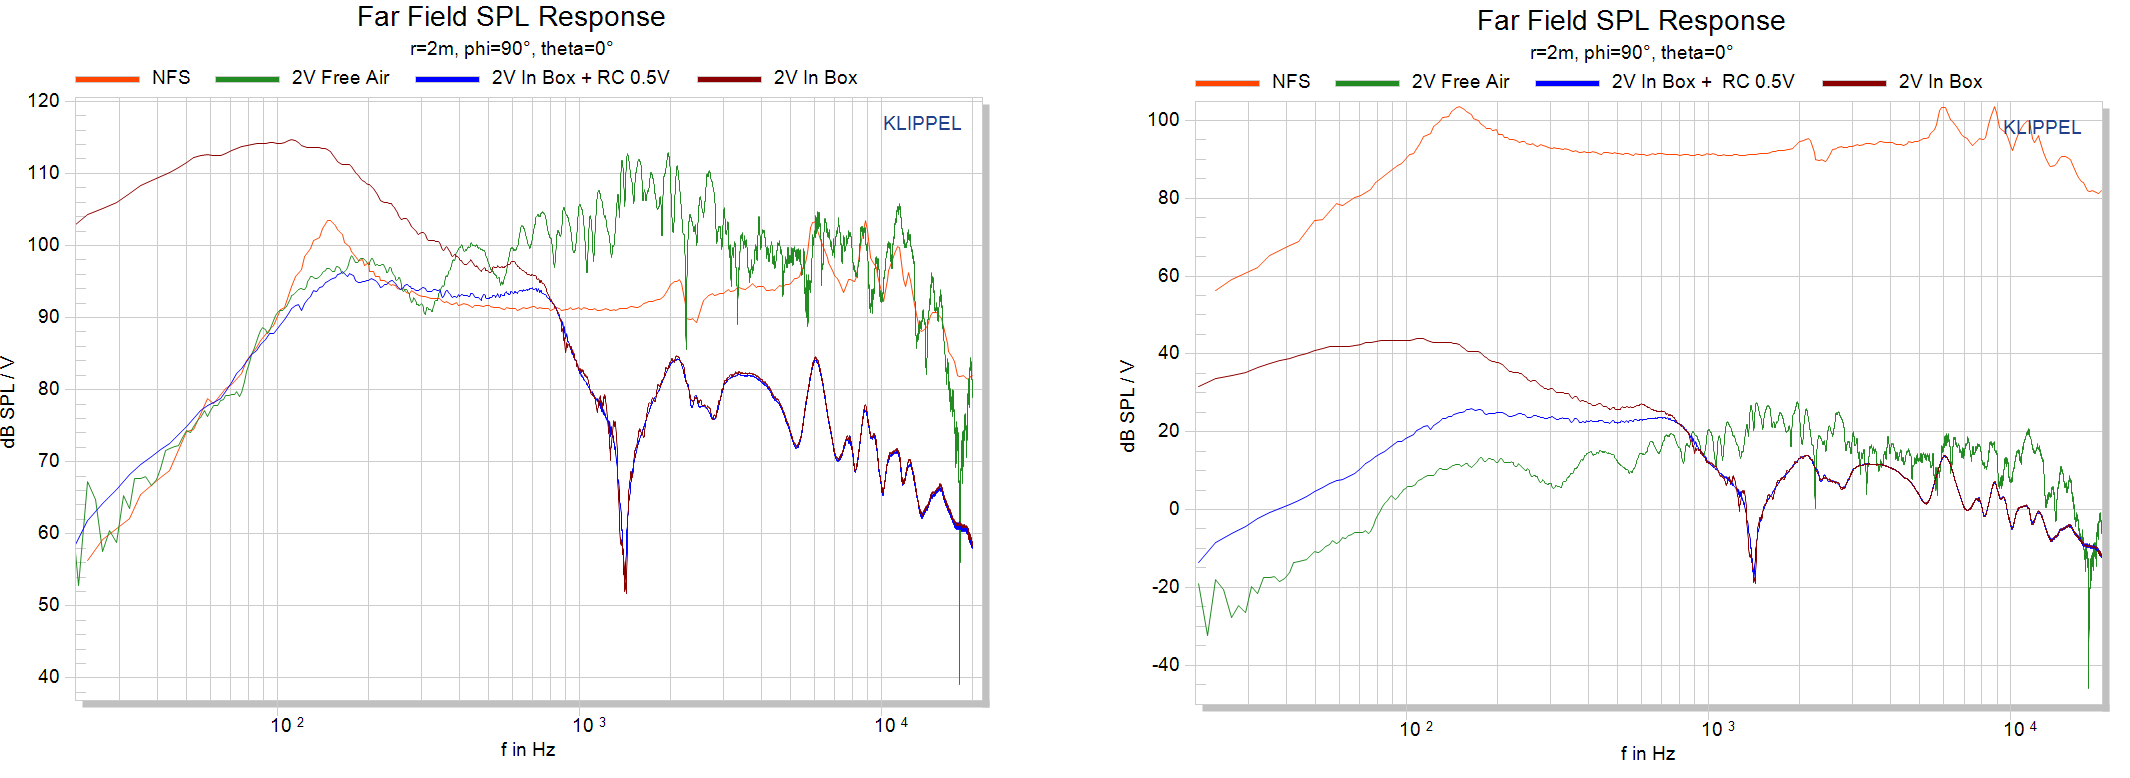
\includegraphics[width=\textwidth]{Appendix/DKeele_FF_All} 
    \captionsetup{hypcap=false} 
	\captionof{figure}{Application of DB Keele method compared with NFS results- Left: shifted curves; Right: non-shifted curves} 
	\label{fig:dbk_fig}
\end{center}




		% Application Notes
\chapter{Application notes}

\section{Baffle measurement}
\label{chap:AN_Baffle}

\end{appendices}

\end{document}